\documentclass{acm_proc_article-sp}

\usepackage[utf8]{inputenc}
\usepackage{cite}
\usepackage{url}
%\usepackage{hyperref}
\usepackage{comment}
\usepackage{listings}
\usepackage{multirow}
\usepackage{hyperref}
\usepackage{graphicx}
\usepackage{subcaption}
\usepackage{tabularx}
\usepackage{color}
\usepackage{multicol}
\usepackage{float}
\usepackage{amsmath}

\urlstyle{same}

\lstset{frame=tb,
  language=C,
  aboveskip=3mm,
  belowskip=3mm,
  frame=single,
  showtabs=false,
  showstringspaces=false,
  columns=flexible,
  basicstyle={\small\ttfamily},
  numbers=left,
  numberstyle=\small,
  numbersep=5pt,
  keywordstyle=\color{blue},
  morekeywords={bool, uint8_t, uint16_t, int8_t},
  commentstyle=\color{green},
  stringstyle=\color{mauve},
  breaklines=true,
  breakatwhitespace=true,
  tabsize=3,
  xleftmargin=12pt,
  xrightmargin=5pt,
  captionpos=b
}
\lstset{emph={%  
    Configuration, Target, Platform, MCU, Interface, Version, 
    Global, ResponseTimeout, InterByteTimeout, Retry,
    Uart, BaudRate, Data, Stop, Parity, 
    Function, Name, EntryPoint, Command, ResponseMatch, Delay, Dependency, DName
    },emphstyle={\color{red}\textbf}%
}%

\begin{document}

%don't want date printed
\date{}

\title{\Large \bf A Software Approach to Protecting Embedded System Memory\\ from Single Event Upsets}

%\subtitle{[Subtitle]
%\titlenote{Sub title footnote}}
%
% You need the command \numberofauthors to handle the 'placement
% and alignment' of the authors beneath the title.
%
% For aesthetic reasons, we recommend 'three authors at a time'
% i.e. three 'name/affiliation blocks' be placed beneath the title.
%
% NOTE: You are NOT restricted in how many 'rows' of
% "name/affiliations" may appear. We just ask that you restrict
% the number of 'columns' to three.
%
% Because of the available 'opening page real-estate'
% we ask you to refrain from putting more than six authors
% (two rows with three columns) beneath the article title.
% More than six makes the first-page appear very cluttered indeed.
%
% Use the \alignauthor commands to handle the names
% and affiliations for an 'aesthetic maximum' of six authors.
% Add names, affiliations, addresses for
% the seventh etc. author(s) as the argument for the
% \additionalauthors command.
% These 'additional authors' will be output/set for you
% without further effort on your part as the last section in
% the body of your article BEFORE References or any Appendices.


\numberofauthors{1} %  in this sample file, there are a *total*
% of EIGHT authors. SIX appear on the 'first-page' (for formatting
% reasons) and the remaining two appear in the \additionalauthors section.
%
\author{
% You can go ahead and credit any number of authors here,
% e.g. one 'row of three' or two rows (consisting of one row of three
% and a second row of one, two or three).
%
% The command \alignauthor (no curly braces needed) should
% precede each author name, affiliation/snail-mail address and
% e-mail address. Additionally, tag each line of
% affiliation/address with \affaddr, and tag the
% e-mail address with \email.
%
% 1st. author
% \alignauthor Jiannan Zhai, Yangyang He, Fred S. Switzer, Jason O. Hallstrom\\
 \alignauthor Author1, Author2, Author3, Author4\\
%    \affaddr{School of Computing, Clemson University, Clemson SC, 29634-0974  USA}\\
    %\affaddr{}
%    \affaddr{ \{jzhai, yyhe, skyler, jasonoh\}@clemson.edu}\\
    \affaddr{ \{author1, author2, author3, author4\}@institution}\\
}
% There's nothing stopping you putting the seventh, eighth, etc.
% author on the opening page (as the 'third row') but we ask,
% for aesthetic reasons that you place these 'additional authors'
% in the \additional authors block, viz.
%\additionalauthors{Additional authors: John Smith (The Th{\o}rv{\"a}ld Group,
%email: {\texttt{jsmith@affiliation.org}}) and Julius P.~Kumquat
%(The Kumquat Consortium, email: {\texttt{jpkumquat@consortium.net}}).}
%\date{30 July 1999}
% Just remember to make sure that the TOTAL number of authors
% is the number that will appear on the first page PLUS the
% number that will appear in the \additionalauthors section.

\maketitle


\begin{abstract}
Radiation from radioactive environments, such as those encountered during space flight, can cause damage to embedded systems. One of the most common examples is the \textit{single event upset} (SEU), which occurs when a high-energy ionizing particle passes through an integrated circuit, changing the value of a single bit by releasing its charge. The SEU could cause damage and potentially fatal failures to spacecraft and satellites. In this paper, we present an approach that extends the AVR-GCC compiler to protect the system stack from SEUs through duplication, validation, and recovery. Three applications are used to verify our approach, and the time and space overhead characteristics are evaluated.
\end{abstract}

% A category with the (minimum) three required fields
%\category{H.4}{Information Systems Applications}{Miscellaneous}
%A category including the fourth, optional field follows...
%\category{D.2.8}{Software Engineering}{Metrics}[complexity measures, performance measures]

%\terms{Terms}

%\keywords{ACM proceedings, \LaTeX, text tagging} % NOT required for Proceedings

\vspace{-10pt}
\section{Introduction}\label{sec:introduction}
\vspace{-5pt}
%Space Exploration has benefited us in almost every aspect of our lives, from communications (e.g., cellphones, internet) to transportation (e.g., GPS) to entertainment (e.g., satellite television and audio service), etc. 
Humans have a longstanding curiosity about outer space. Since the launch of the first artificial satellite, Sputnik 1~\cite{sputnik1}, in 1957, over 6,000 satellites have been launched into space. There are more than 1,000 operating satellites in orbit around Earth~\cite{satellite:total} today, and an estimated 1,200 satellites will be launched over the next decade~\cite{satellite:next10years}. As of 2012, more than 130 manned spacecraft have been launched by the United States~\cite{space:shuttle:list}. There are currently two operational space stations, and seven more are planned over the next decade~\cite{space:station:tiangong2}\cite{space:station:almaz}\cite{space:station:opsek}\cite{space:station:tiangong3}. Given the high cost and vital importance of spacecraft rovers and satellites, as well as their increasing functionality and complexity, the hardware and software reliability requirements are stringent.

One of the most important factors that affect the reliability of spacecraft (and other equipment) is the quality of the constituent embedded components which control telemetry systems, command systems, attitude control systems, and more~\cite{fundamentals:space}. For example, the MSX (Midcourse Space Experiment) spacecraft, launched in the mid-1980s, was equipped with 54 embedded processors, running more than 275,000 lines of code, managing 19 subsystems~\cite{fundamentals:space}. Embedded software failures can cause serious consequences in this context. In 1996, the Ariane 5 spacecraft, which took 10 years and 7 billion (US) dollars to build, crashed due to the failure of the Flight Control Subsystem~\cite{ariane5}.

The environment outside the Earth's atmosphere is highly radioactive. The radiation is generated mainly by the sun and other stars and can cause damage to semiconductor devices~\cite{fundamentals:space}. One of the most common types of damage caused by radiation is the \textit{single event upset} (SEU). Extremely small electronic components (i.e., tens of nanometers~\cite{intel:chip:size}) are used in modern integrated circuitry; the components cannot carry much charge. As a result, one high-energy ionizing particle passing through an integrated circuit can release enough charge to change the state of a binary digit, causing a stored bit to change to its opposite value (i.e., a 0-bit can become a 1-bit, and vice-versa~\cite{fundamentals:space}). The damage caused by an SEU can range from system malfunction to system crash.
% This phenomenon is known as a \textit{Single Bit Upset}. It has also been observed that two or more stored bits can be changed by one high-energy particle striking at certain angles of incidence, known as a \textit{Multiple Bit Upset} (MBU). The damage caused by an SEU (or MBU) can range from system dysfunction to system crash, both of which are intolerable for spacecraft embedded systems. %Modern approaches used to prevent and correct SEU errors often introduce additional hardware and software to the target system. Systems designed to be used in space often contain processors fabricated using Silicon On Insulator technology, which effectively reduces the size of the processor, and therefore reduces the vulnerable area that a highly-charged particle could strike.Triple modular redundancy (TMR)~\cite[p.645]{fundamentals:space} uses three identical systems (either physically or temporally duplicated) to simultaneously perform identical tasks, where the correct result is then decided by a majority vote. Due to the inherent randomness of Single Event Upsets, the chance that two charged particles would strike parallel locations in two different systems at the same time is incredibly low, making TMR a very popular practice in spite of the memory expense. Another popular SEU correction method is the use of codes such as the Hamming Code to correct bit errors~\cite{Shirvani2001EDAC}. However, most of these processes are supplemented by periodic memory scrubbing and hardware watchdog timers used to check execution flow and abnormal program executions caused by SEUs~\cite[p.648]{fundamentals:space}. 

Modern approaches used to prevent and correct SEU errors often introduce additional hardware to the target system. In this paper, we present a {\em software-only} approach that detects and corrects SEUs in RAM. The paper focuses on the system stack, which is the most important and dynamic region in memory. The system stack is protected by injecting customized code into the target assembly generated by AVR-GCC. After injection, each callee computes and saves the checksum of its caller's current stack frame and duplicates the caller's stack frame when the callee enters its function body. Before the callee returns, it verifies the stack frame of the caller using the saved checksum and overwrites the stack frame using the duplicate, if an SEU is detected. Our approach changes the target system software and does not introduce additional hardware. Since our approach operates at the assembly level, it is language and application neutral. To demonstrate our approach, an AVR microprocessor, the ATmega644~\cite{atmel:avr}, is used in the paper. 

The main contributions of our work are as follows: (i) We present an approach that protects the system stack by injecting assembly code at the beginning and end of each application function. (ii) We present an implementation of the approach, using the popular AVR architecture as a target. (iii) We verify the protection efficacy of our approach and evaluate performance in terms of space and speed overhead using three applications with different stack usage patterns.

%(i) We summarize the key operations regarding code injection by analyzing the assembly code generated by AVR-GCC with the optimization level set to \texttt{none}. Each operation represents a phase in the execution sequence, such as initializing the function stack, function return, etc. (ii) We present an algorithm used to scan the AVR assembly code, and categorize operations performed by each line of the assembly code based on the assembly metadata we designed. Based on scan results, customized assembly code is injected into the target assembly code, handling register saving and restoring, checksum computation, memory duplication, etc. (iii) Finally, three (?) real-world applications are considered to verify our approach, and evaluate its performance using an AVR simulator.

{\bf Paper Organization.} Section \ref{sec:related_work} summarizes key elements of related work. Section \ref{sec:background} provides background related to our approach, including the microprocessor architecture, AVR function call process, and AVR toolchain. Section \ref{sec:design} presents the design and implementation of our approach. Section \ref{sec:evaluation} presents an evaluation of the approach, with an emphasis on ROM size and execution speed overhead. Finally, Section \ref{sec:conclusion} concludes with a summary of contributions and pointers to future work.
\section{Related Work}\label{sec:related_work}

Prior work on single event upset mitigation spans two categories:
First, robustness at the device level may be improved by building the hardware in such a way that radiation does not cause upset events. 
Common hardware modifications include physical shields, protective insulation, and error correcting latches.
Second, design level robustness may be improved by incorporating libraries and software designed to protect from single event upsets through the use of Hamming or other codes, or triple modular redundancy.

\subsection{Device-Level Robustness}

One of the primary methods of device-level radiation hardening is to fabricate processors using Silicon on Insulator (SOI) technology.
In this process, transistors are placed on a thin layer of silicon, which is then placed on top of an insulator, reducing the capacitance of the switches and the size of processors~\cite{Celler2003SOI}.
Reducing processor size effectively reduces the area over which highly-charged particles can strike, statistically reducing the likelihood of impacts, and therefore errors.

Irom et al.~\cite{Irom2002SOI} compare SEU error rates in  SOI microprocessors to conventional microprocessors.
They subject both types of microprocessors to proton impacts within a cyclotron, and to heavy-ion impacts within an accelerator, both of which are known to cause SEUs in processors.
From these tests, Irom et al. conclude that due to the significant reduction of cross sections in SOI microprocessors, SEU rates are lower than those in commercial microprocessors.

She et al.~\cite{She2012Latch} improve the design of conventional latches by implementing an error detection circuit and integrated multiplexer.
While conventional latches are susceptible to voltage changes caused by SEUs, the proposed latch uses an error detection circuit that checks for faults using the precharge and discharge operations.
The latch uses a multiplexer to output a corrected signal based on the fault detected by the error detection circuit.
The authors found that the proposed latch introduces little overhead and offers good performance, as well as better SEU protection than conventional latches.

\subsection{Design-Level Robustness}

The most popular methods of radiation hardening are at the design level, foregoing the need to modify the hardware, thereby allowing the use of commercial microcontrollers.
Some of these methods involve parity bits and linear error-correcting codes~\cite{ErrorCorrectingCodes}, such as the Hamming code, which correct bit errors by storing extra information about data in larger blocks.
Alternately, Triple Modular Redundancy (TMR)~\cite{TMR} is a voting-based approach that prevents errors by implementing three systems, and then using the common result.
The motivation is that the likelihood of two single event upsets occurring at precisely the same time, in the same geographic location, in two different devices, is incredibly low, making TMR popular in spite of the added expense.
While this method can be implemented via hardware (such as in RAID~\cite{RAID}), it is also effective as a software-only strategy.

Shirvani et al.~\cite{Shirvani2001EDAC} examine a set of error detection and correction (EDAC) methods.
These methods detect and subsequently correct errors in memory, such as those caused by SEUs.
EDAC methods come in both hardware and software forms.
In scenarios where hardware-based approaches are cost prohibitive, software-based methods work well.
The authors found that the reliability of software-based methods tends to decrease over time more rapidly than hardware-based methods.
However, the rate of reliability loss is low enough to still be more cost effective than hardware-based methods.
% but at a rate that it would still be cost-efficient to forgo hardware hardening in favor of software-based error correction.
Four software-based coding schemes were considered, comprising Hamming, Cyclic, Parity, and Reed-Solomon codes.
The authors found that most EDAC implementations can be improved by periodically scrubbing (completely cleaning) memory.
%EDAC is simply a blanket term for most of the error detections and error recovery methods outlined in this article, and this Stanford tech report goes into detail on many of them, providing useful statistical analysis.

Mhatre and Aras~\cite{mhatreSeuTmr} present a design for the on-board computer of the COEP Student Satellite, a HAM communication pico-satellite. 
SEU protection on the satellite involves the implementation of Hamming codes, Triple Modular Redundancy, and watch-dog software.
In the Hamming code, each 32-bit instruction is coded in the form of a 38-bit codeword, where the redundant bits are used for parity.
Single bit errors are corrected by comparing the parity values with pre-calculated values.
Triple Modular Redundancy is used in storing and protecting these parity values, saving space by not implementing TMR over the entire instruction memory.
This extra storage increases program memory requirements by 75\%, rather than the 200\% increase required by a full implementation of TMR.
The watch-dog software prevents other errors by automatically escaping system crashes.


Similarly, Dutton and Stroud present a design implemented in configurable logic blocks for SEU detection and correction in the configuration memory of field programmable gate arrays (FPGAs)~\cite{CATA09seuonVirtex}.
The architecture of the Xilinx Virtex FPGA is modified to implement an SEU controller that uses Hamming codes and parity values to detect and correct single bit errors in memory.
This combination of Hamming and parity can also detect multiple bit upsets, but correction is still not possible.
The benefits include the protection of the controller from SEUs and the high speed of error detection and correction, as compared to other methods.

\vspace{-20pt}
\section{Background}\label{sec:background}
\vspace{-10pt}
While our approach is architecture neutral, our implementation is based on the Atmel AVR toolchain and focuses on AVR microprocessors. In this section, we survey the stack frame, function call process, and the AVR Toolchain optimization levels.
\vspace{-10pt}
\subsection{Stack Frame}
\vspace{-10pt}
The stack consists of stack frames, each corresponding to a function call. A stack frame is created when a function is called, and freed when the function returns. For example, as shown in Figure \ref{fig:stack_frame}, when the \textit{main} function calls the \textit{foo} function, a stack frame will be created for \textit{foo}. First, the return address of \textit{main} will be pushed to the stack, followed by the conflict registers. Next, the local variables and parameters will be pushed to the stack in reverse order of declaration. The stack frame spans the return address through the first parameter. The stack frame pointer, Y, now points to the next available address in the stack. When \textit{foo} finishes execution, the stack frame will be freed, and the stack frame pointer will point back to the position where the return address of the previous stack frame was stored.
\vspace{-15pt}
\begin{figure}
\centering
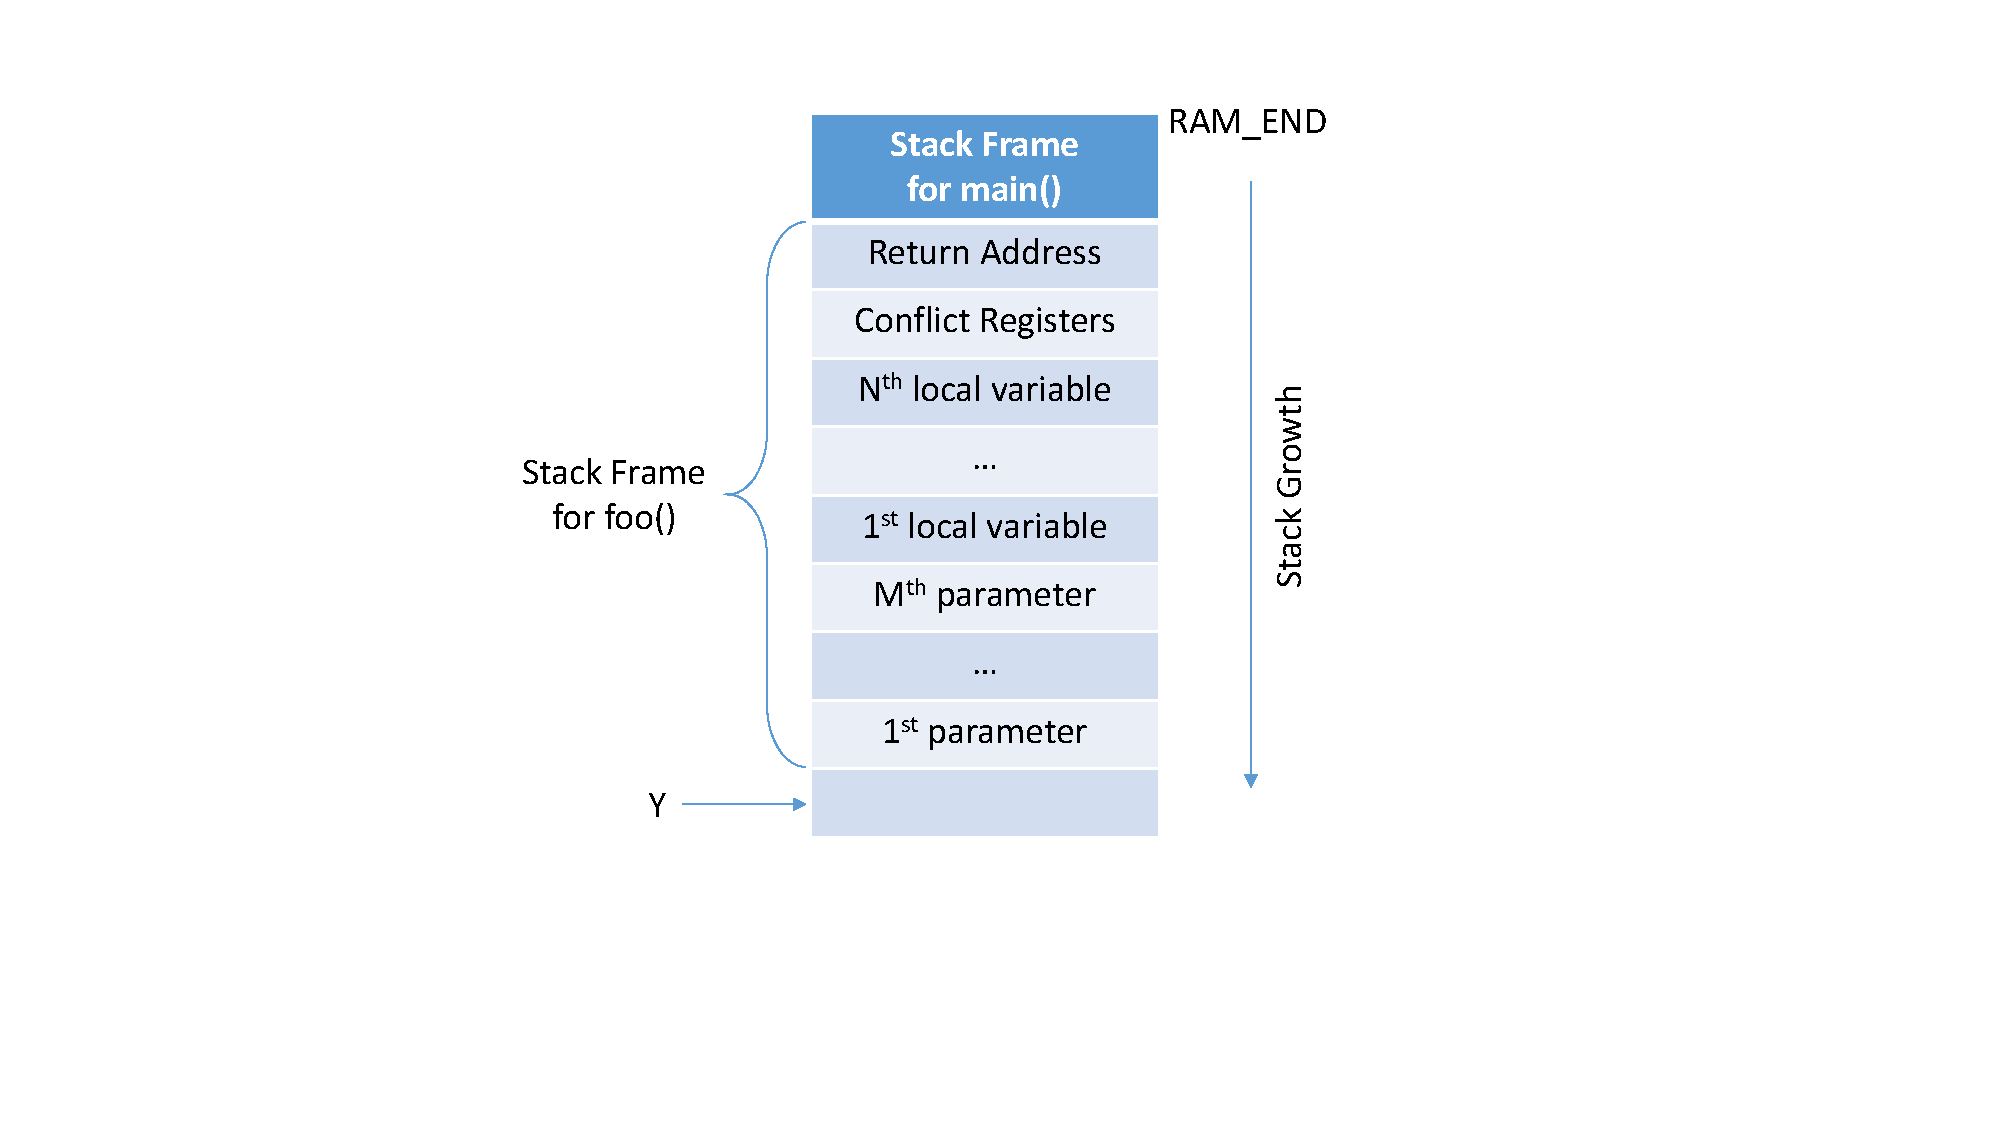
\includegraphics[scale=0.55]{figures/stack_frame_v2.pdf}
\vspace{5pt}
\caption{AVR Stack Frame}
\label{fig:stack_frame}
\end{figure}
\vspace{-20pt}
\vspace{-10pt}
\subsection{Function Calls}
\vspace{-10pt}
All function calls follow the same process and use the system stack to perform most operations, as illustrated in Figure \ref{fig:original_function_operation}. Figure \ref{fig:original_function_operation_process} explains the execution process when a function is called, and Figure \ref{fig:original_function_operation_stack} shows the associated stack changes after each operation is performed. Each rectangle represents two bytes in the stack. The numbers below each stack denote the operation(s) that changed the stack. \texttt{SP} denotes the stack pointer, and \texttt{Y} denotes the stack frame pointer. When a function is called, the return address is automatically pushed onto the stack by one of the function call instructions, \texttt{call}, \texttt{rcall}, or \texttt{icall} (step 1). After the stack frame pointer is pushed (step 2), the stack frame of the function is created by changing the stack pointer and stack frame pointer (step 3). The arguments and local variables are then pushed onto the stack (step 4), and the function begins executing (step 5). The arguments and local variables are released after the function finishes its execution (step 6), and the stack frame pointer is restored (step 7). Finally, the function returns (step 8). The return address is popped and used when one of the function return instructions, \texttt{ret} or \texttt{reti}, is called.
\begin{figure}
	\centering
	\begin{subfigure}[b]{0.4\columnwidth}
		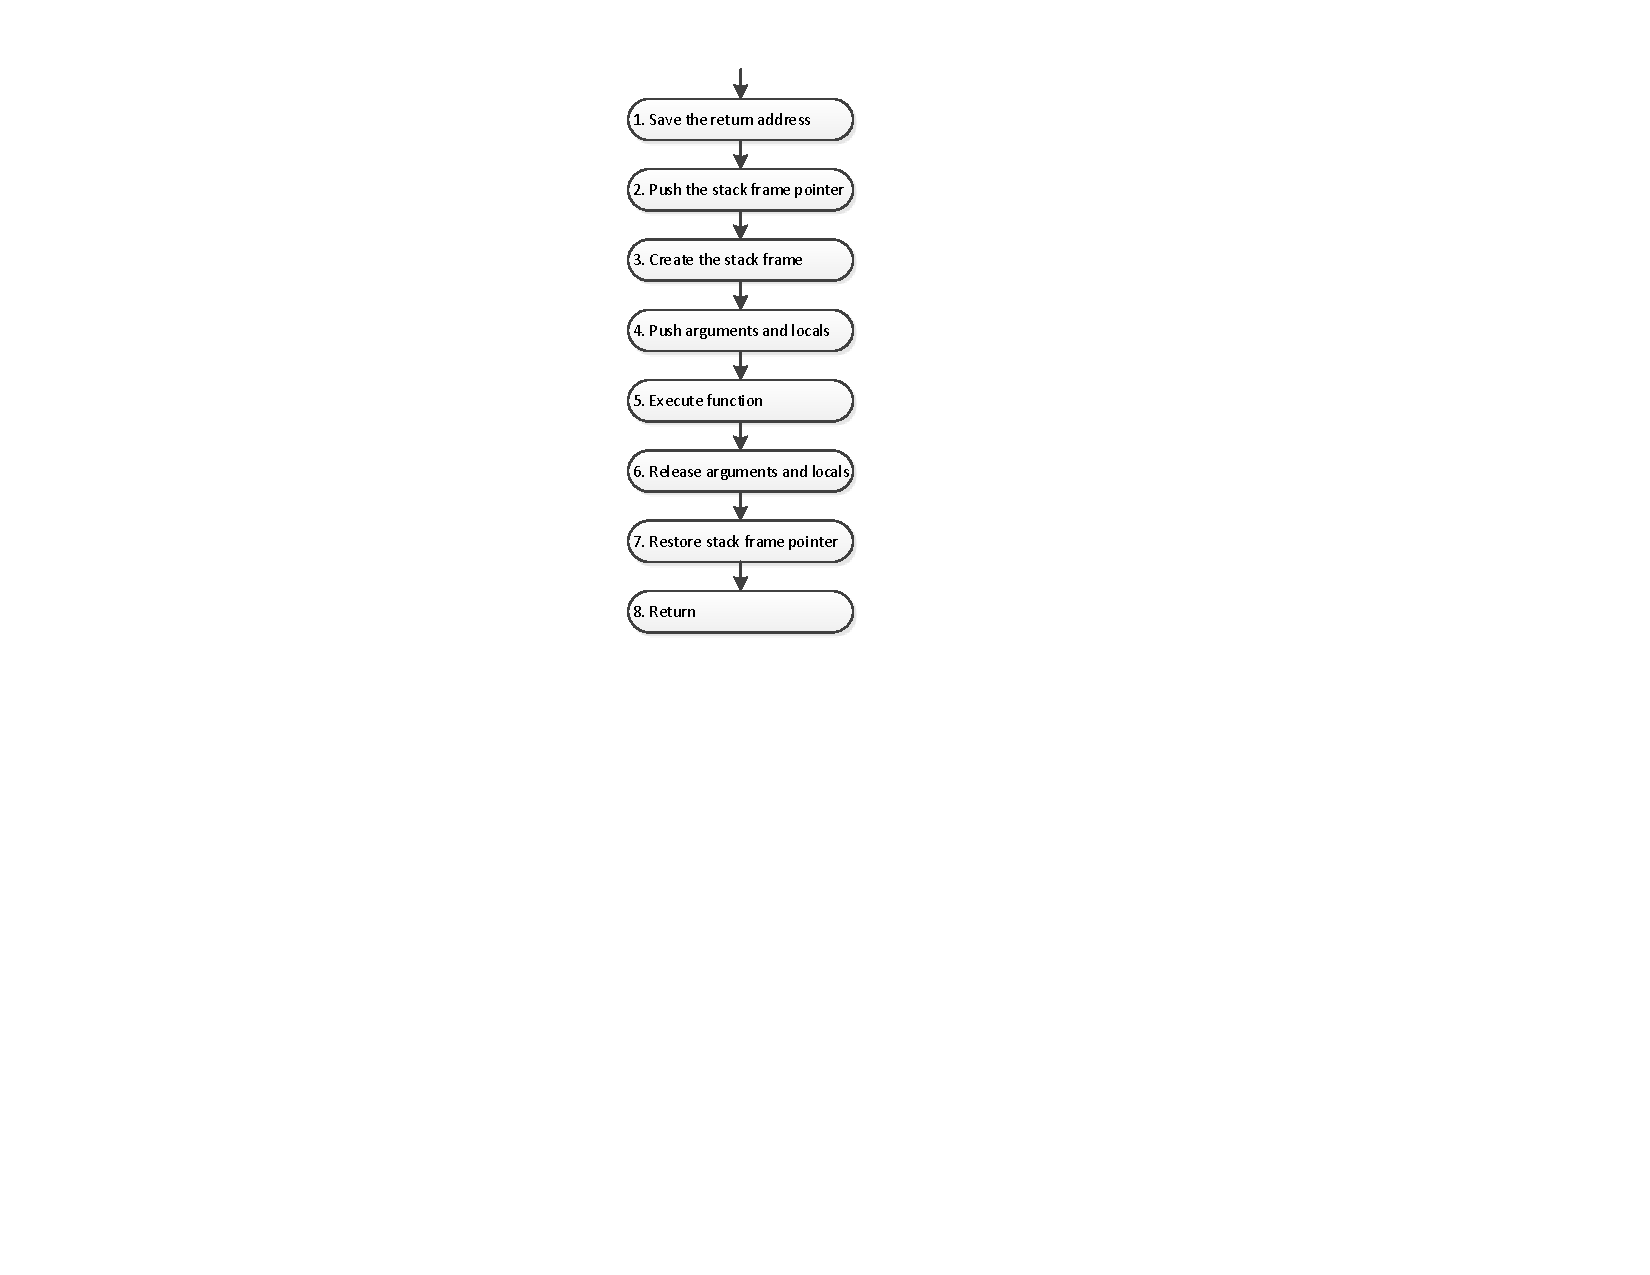
\includegraphics[width=\textwidth, height=12cm]{figures/original_function_operations_process_v3}
		\caption{Process}
		\label{fig:original_function_operation_process}
	\end{subfigure}~
	\begin{subfigure}[b]{0.6\columnwidth}
		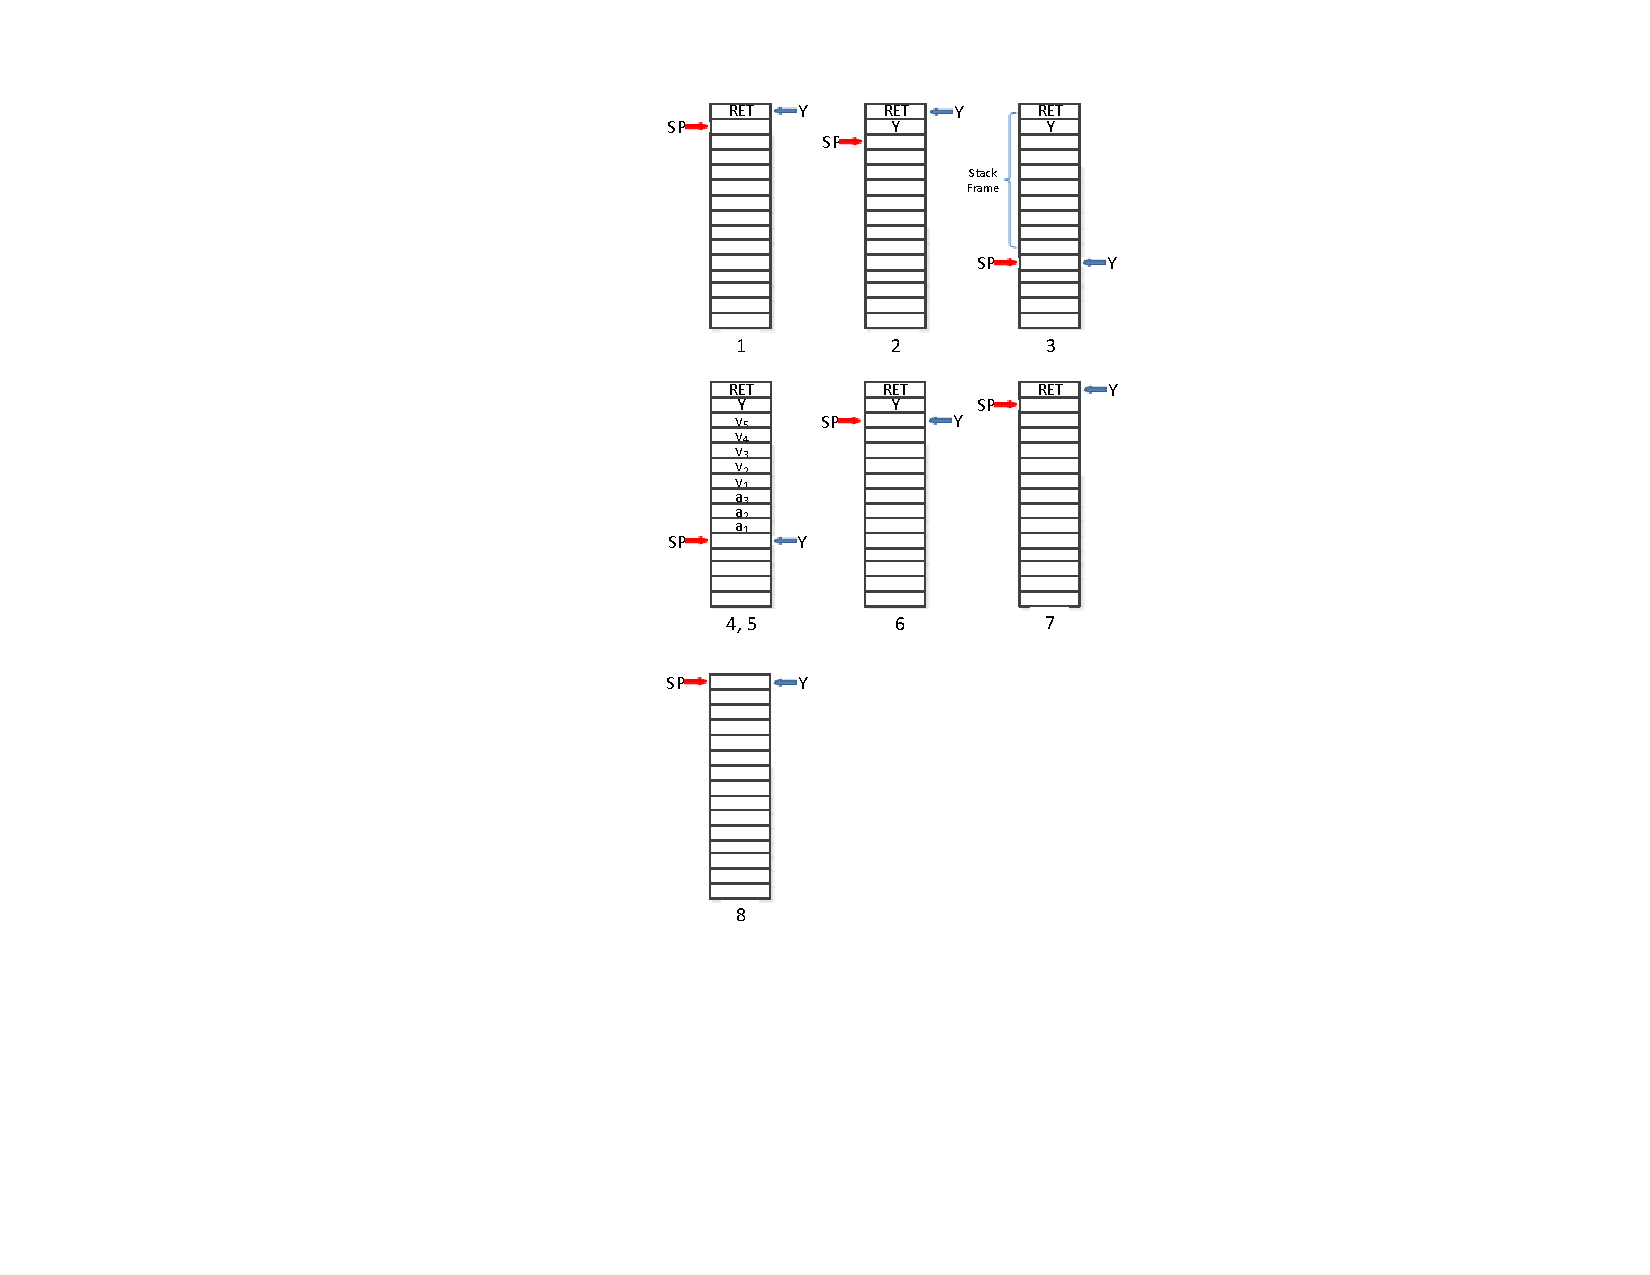
\includegraphics[width=\textwidth, height=11.5cm]{figures/original_function_operations_stack_v2}
		\caption{Stack}
		\label{fig:original_function_operation_stack}
	\end{subfigure}
	%	\vspace{5pt}
	\caption{Function Execution}\label{fig:original_function_operation}
\end{figure}
\vspace{-15pt}
\vspace{-10pt}
\subsection{AVR Toolchain Optimization Levels}
\vspace{-10pt}
The AVR GCC toolchain is used in our approach. It provides 5 optimization levels, each providing different optimization options. The exception is -O0, which offers no optimization\cite{hoste2008cole}. Our approach is based on modifying unoptimized assembly code generated with the -O0 option. This option makes it more convenient for developing, debugging, and evaluating our approach. However, we plan to extend our approach to other optimization levels in future work.


\begin{comment}
\subsection{AVR Architecture}

AVR microprocessors are based on a modified Harvard architecture~\cite{argade1996apparatus}, which stores instructions and data in physically separate memories, flash memory and SRAM, respectively. Instructions and data are accessed concurrently through separate memory buses. Flash memory is non-volatile and offers high capacity, but slow access speed, and is used to store executable programs composed of AVR instructions. The SRAM is volatile and offers low capacity, but fast access speed, and is used to store data used by the executable programs at runtime. The ATmega644 includes 64KB of flash memory, 4KB of SRAM, a 16-bit instruction bus, and an 8-bit data bus.

\subsubsection{AVR SRAM}

The on-board SRAM of the ATmega644 has an address range of 0x0100 to 0x10FF, as shown in Figure \ref{fig:ram_map}. The SRAM is partitioned into sections, each used to store different types of data. The \textit{.data} section is used to store initialized static variables and global variables. The \textit{.bss} section is used to store uninitialized static and global variables. The pre-allocated SRAM usage is the sum of the sizes of the .data and .bss sections. The remaining space in SRAM is shared by the heap and stack sections. The \textit{heap} section is used to store dynamically allocated memory, e.g. when \textit{malloc()} is called~\cite{goldt1995linux}. The heap grows ``upward'', towards the higher address range. The \textit{stack} section is used to store a return address, actual parameters, conflict registers, local variables, and other information. The stack grows ``downward'', from \textit{RAM\_END}, address 0x10FF, towards the lower address range.
\begin{figure}
\centering
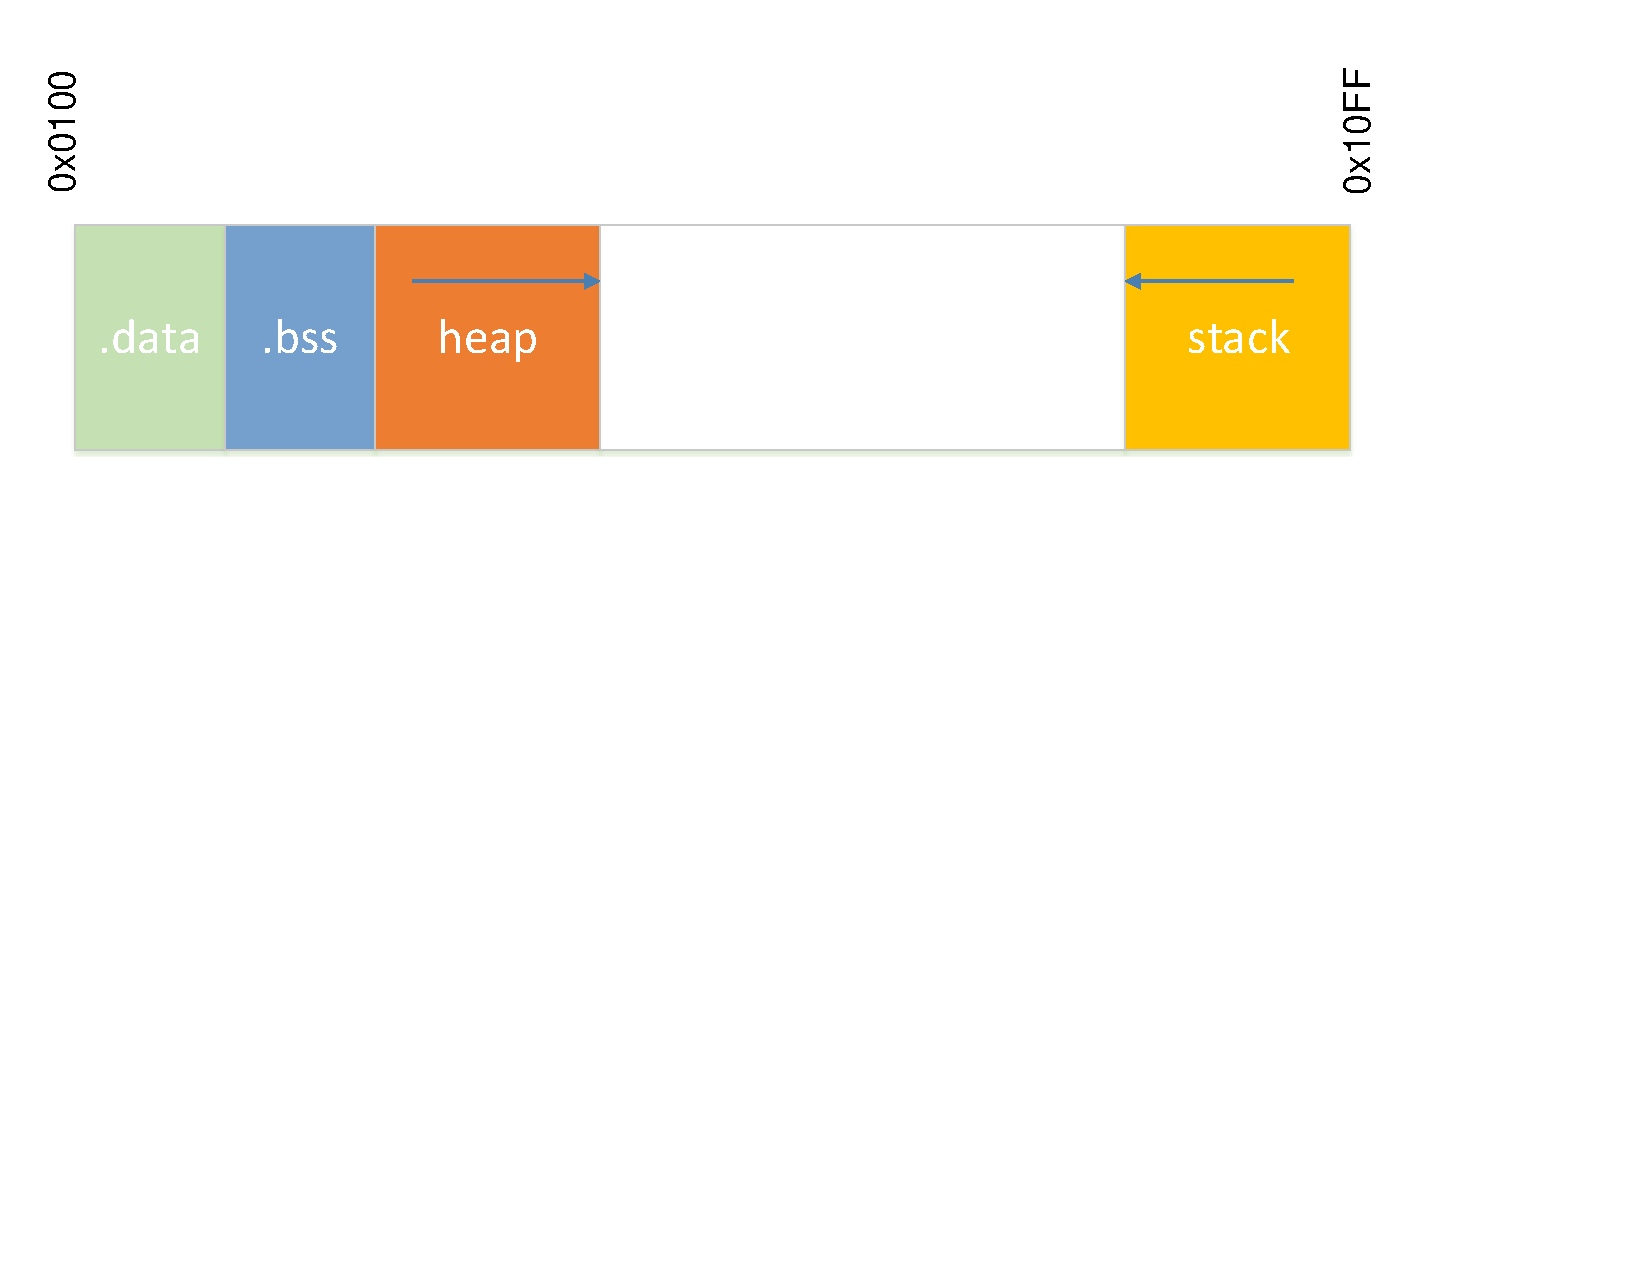
\includegraphics[width=0.5\textwidth]{figures/Memory_model.pdf}
\caption{AVR RAM Map}
\label{fig:ram_map}
\end{figure}

\subsubsection{Stack Frame}

The stack consists of stack frames, each corresponding to a function call. Each stack frame is created when a function is called, and freed when the function returns. For example, as shown in Figure \ref{fig:stack_frame}, when the \textit{main} function calls the \textit{foo} function, a stack frame will be created for \textit{foo}. First, the return address of \textit{main} will be pushed to the stack, followed by the conflict registers. Next, the local variables and parameters will be pushed to the stack in reverse order of their declarations. The stack frame spans the return address through the first parameter. The stack frame pointer, Y, now points to the next available address in the stack. When \textit{foo} finishes execution, the stack frame will be freed, and the stack frame pointer will point back to the position where the return address of the previous stack frame was stored.

\begin{figure}
\centering
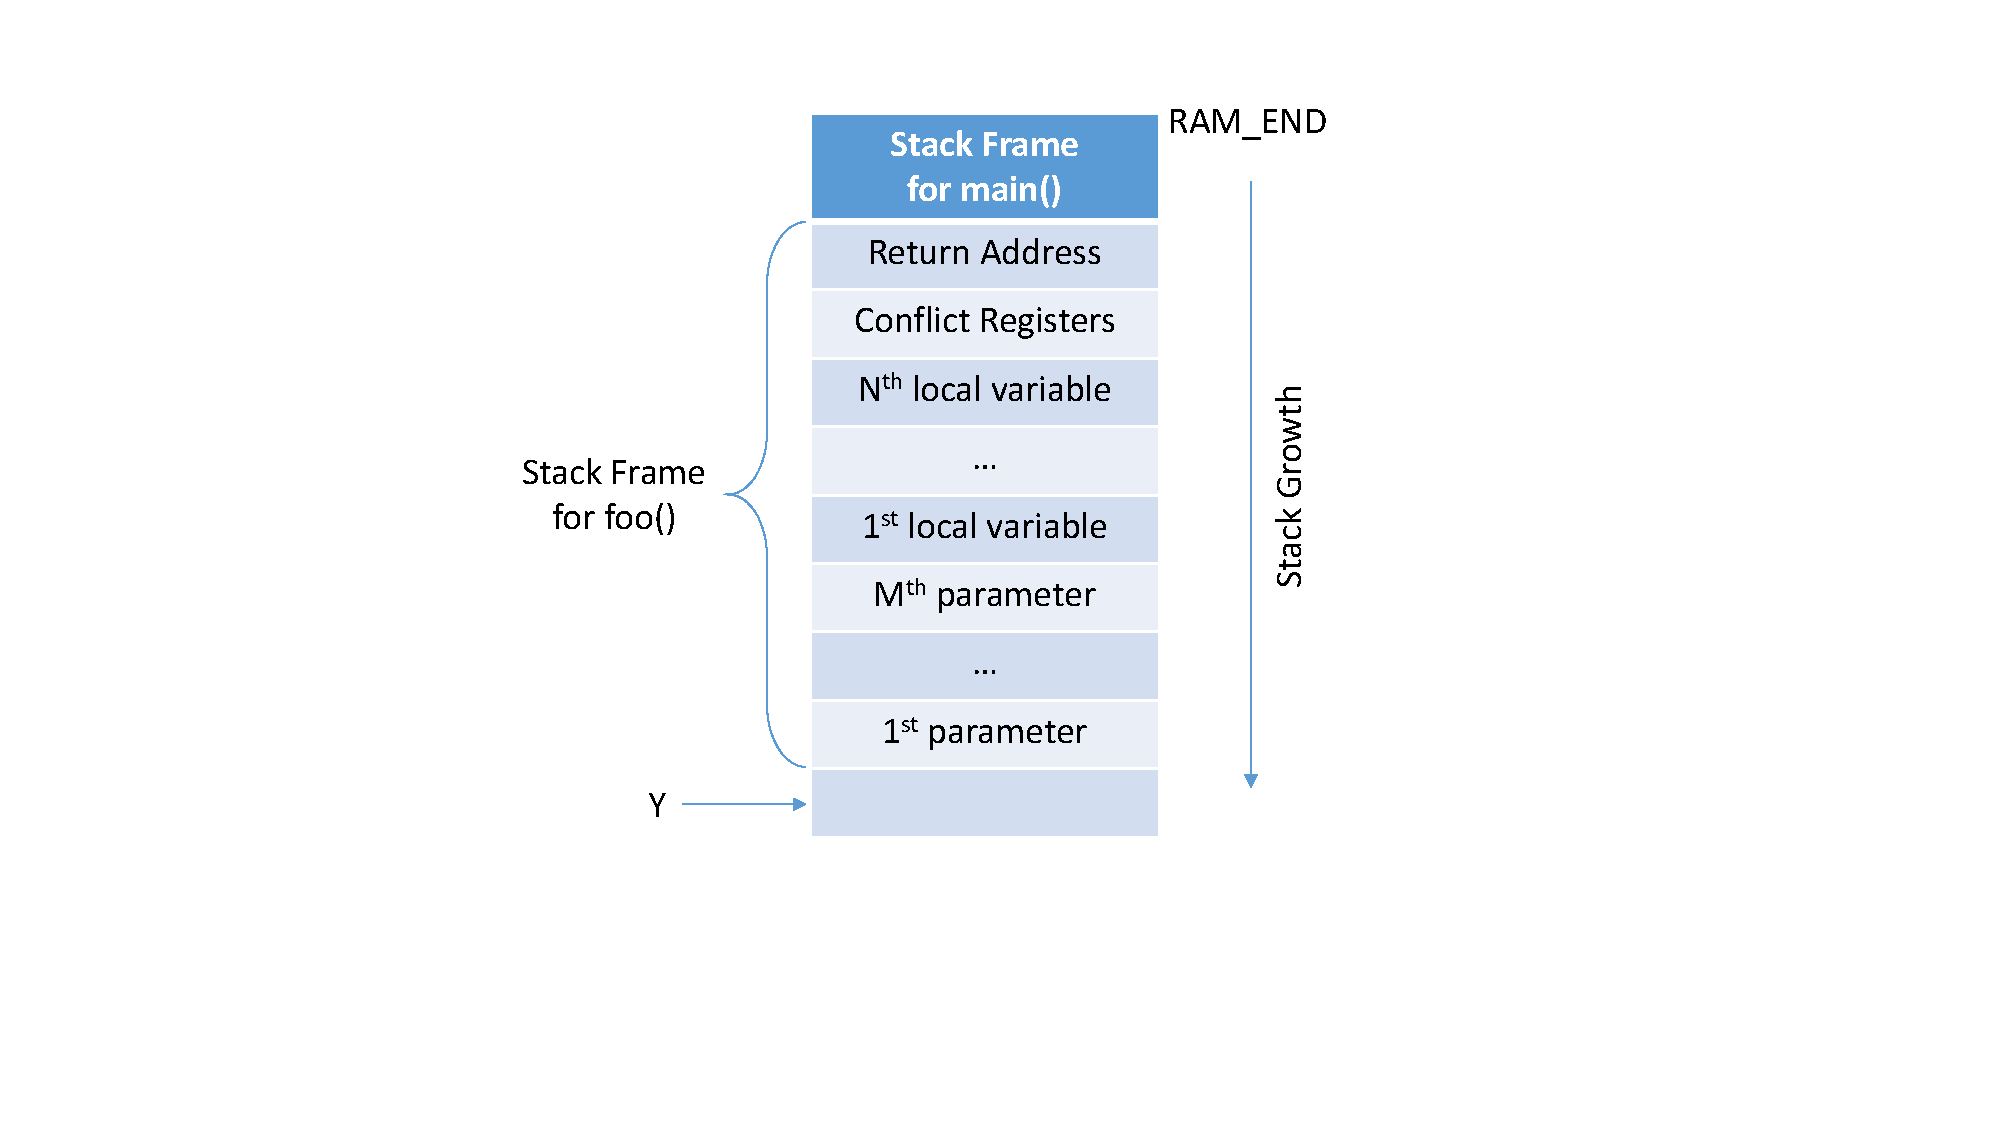
\includegraphics[scale=0.55]{figures/stack_frame_v2.pdf}
\caption{AVR Stack Frame}
\label{fig:stack_frame}
\end{figure}

\subsubsection{Registers}

AVR microprocessors have two types of registers, general-purpose registers and I/O registers. 

General-purpose registers are used for arithmetic operations, such as adding, subtracting, and comparing numbers, as well as indexing and setting long jump destinations. The ATmega644 has 32 general-purpose registers, R1 through R32, which are mapped into the first 32 locations of the RAM space, and can be directly used in assembly commands. Some general-purpose registers are used for special purposes; for example, R29 and R28 store a 16-bit address, the Y pointer, to indicate the top of the current stack frame. (The use of the Y pointer will be explained in the next subsection). The use of these registers is compiler-dependent. For example, AVR-GCC uses R24 and R25 to store the return value of each function call. We attempt to limit the number of registers manipulated by our approach to reduce the cost of saving and restoring the conflict registers.

The I/O registers are used to control the internal peripherals of the AVR microprocessor.
The ATmega644 has 64 I/O registers, mapped into the next 64 locations of the SRAM space, \textit{0x20} through \textit{0x5F}. Again, some I/O registers are used for special purposes; for example, AVR-GCC uses \textit{0x3E} and \textit{0x3D} as the stack pointer (SP), which indicates the current top of the stack.

\subsection{Function Calls}

All function calls follow the same process and use the system stack to perform most operations, as illustrated in Figure \ref{fig:original_function_operation}. Figure \ref{fig:original_function_operation_process} explains the execution process when a function is called, and Figure \ref{fig:original_function_operation_stack} shows the associated stack changes after each operation is performed. Each rectangle represents two bytes in the stack. The numbers below each stack denote the operation(s) that changed the stack. \texttt{SP} denotes the stack pointer, and \texttt{Y} denotes the stack frame pointer. When a function is called, the return address is automatically pushed onto the stack by one of the function call instructions, \texttt{call}, \texttt{rcall}, or \texttt{icall} (step 1). After the stack frame pointer is pushed (step 2), the stack frame of the function is created by changing the stack pointer and stack frame pointer (step 3). The arguments and local variables are then pushed onto the stack (step 4), and the function begins executing (step 5). The arguments and local variables are released after the function finishes its execution (step 6), and the stack frame pointer is restored (step 7). Finally, the function returns (step 8). The return address is popped and used when one of the function return instructions, \texttt{ret} or \texttt{reti}, is called.

\begin{figure}[h]
        \centering
        \begin{subfigure}[b]{0.4\columnwidth}
                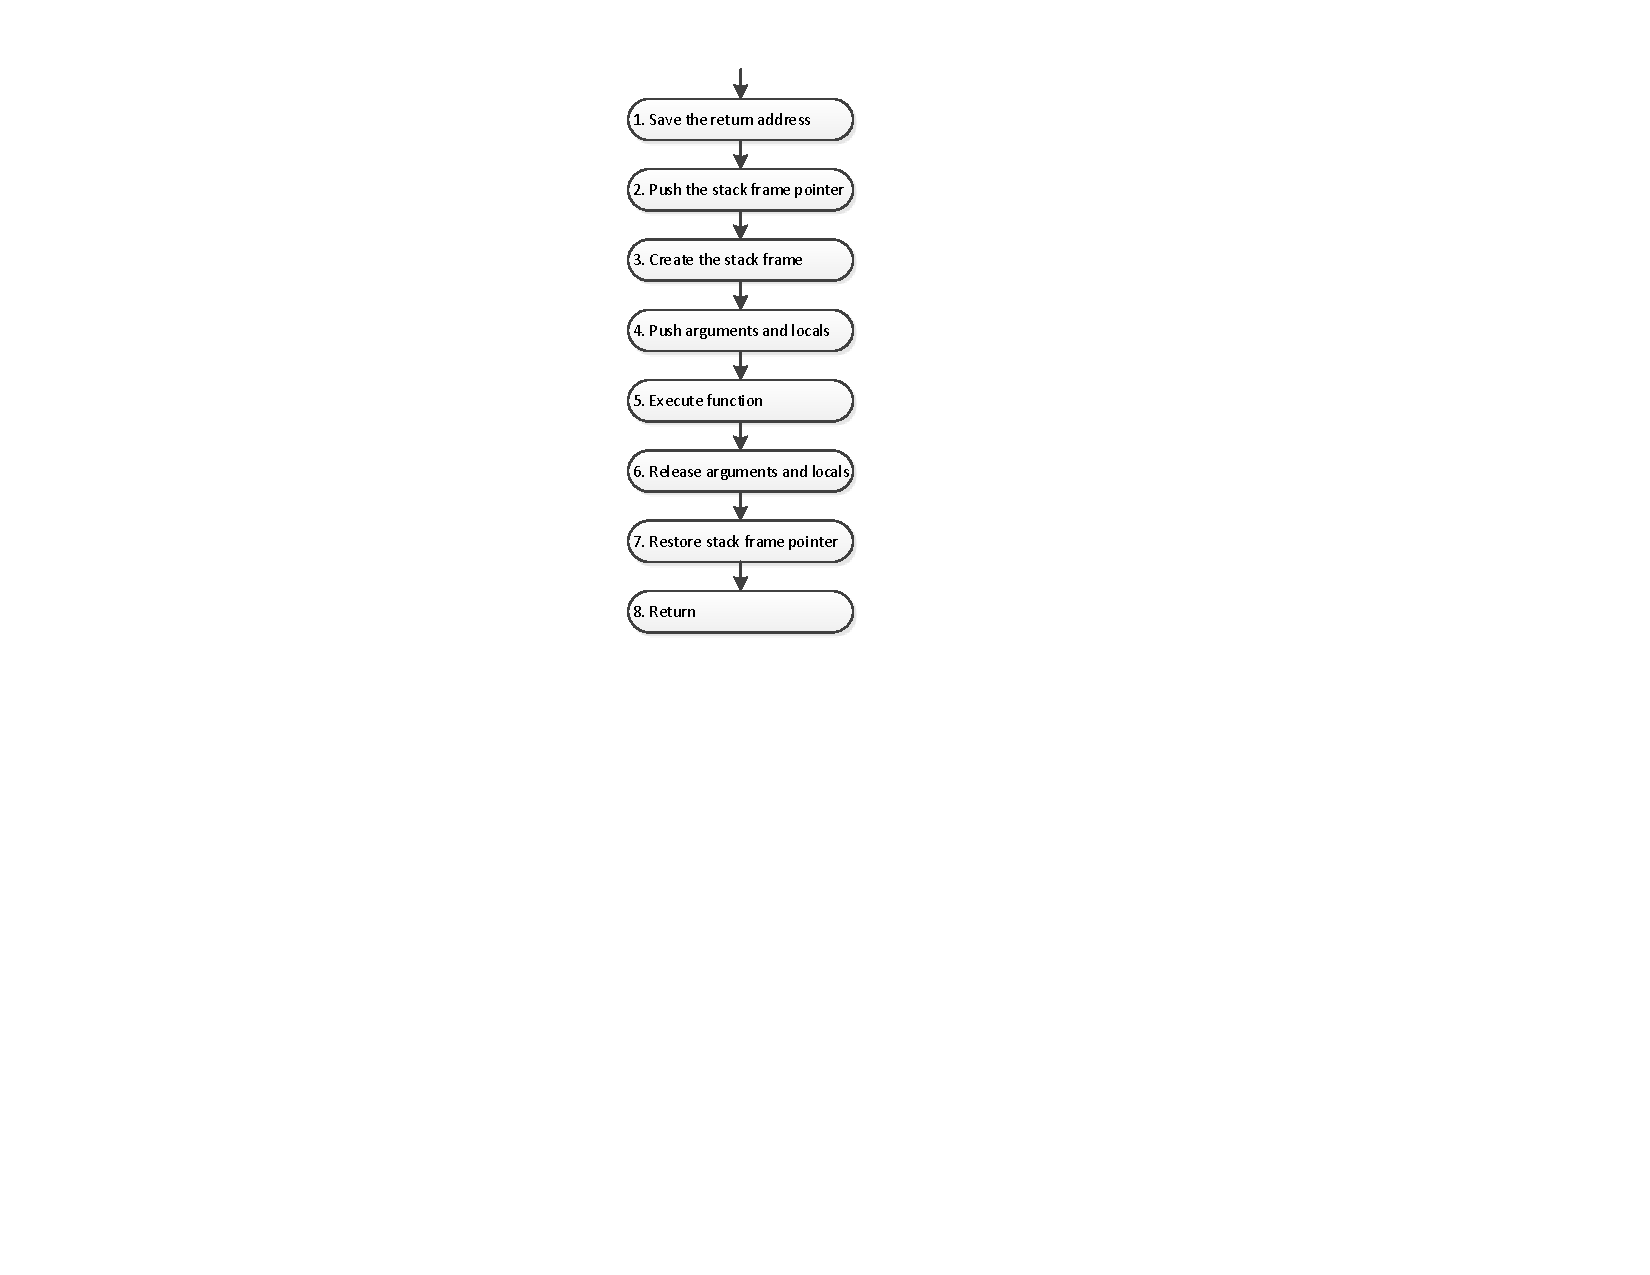
\includegraphics[width=\textwidth, height=12cm]{figures/original_function_operations_process_v3}
                \caption{Process}
                \label{fig:original_function_operation_process}
        \end{subfigure}~
        \begin{subfigure}[b]{0.6\columnwidth}
                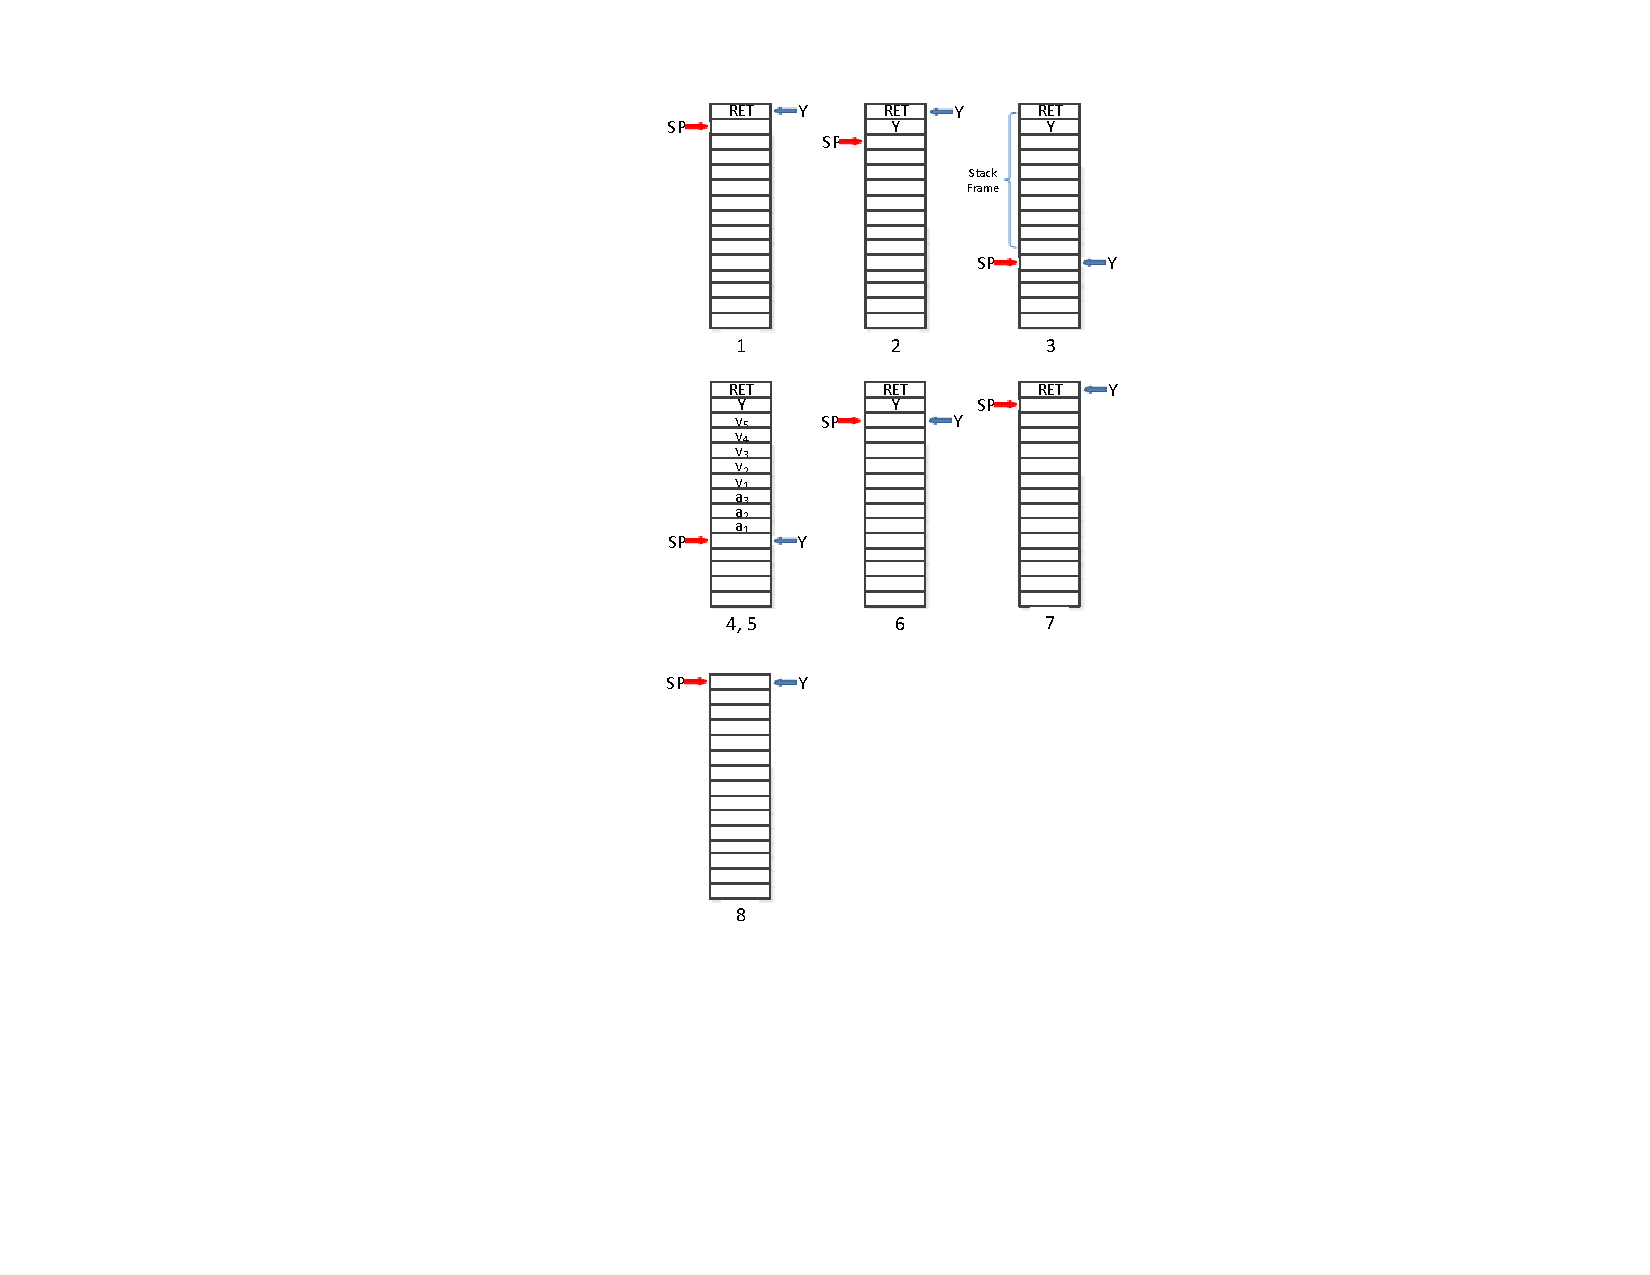
\includegraphics[width=\textwidth, height=11.5cm]{figures/original_function_operations_stack_v2}
                \caption{Stack}
                \label{fig:original_function_operation_stack}
        \end{subfigure}
        \caption{Function Execution}\label{fig:original_function_operation}
\end{figure}

\subsection{Atmel AVR Toolchain}

The Atmel AVR toolchain is a collection of tools used to generate executable programs for AVR microprocessors. The toolchain consists of the following tools.

\begin{itemize}

\item \textit{avr-gcc}, an extension of GNU GCC, is a cross compiler, which translates high-level C or C++ code to assembly code for AVR microprocessors.

\item \textit{avr-as} is an assembler, which translates AVR assembly code to an object file.

\item \textit{avr-ld} is a linker, which uses a linker script to combine object modules into an executable image suitable for loading into the flash memory of an AVR microprocessor. By using a customized linker script, the default locations and sizes in SRAM can be changed. New memory sections may also be added~\cite{sram}.

\item \textit{avr-libc} is a standard C library, which contains standard C routines, as well as additional AVR-specific library functions.

\end{itemize}

As a matter of convenience, the AVR toolchain can be used to compile, assemble, and link C programs in a single command. However, in order to modify the assembly code of an AVR application and use a customized linker script, these steps are performed individually.


AVR GCC provides 5 optimization levels, -O0, -O1, -O2, -O3, and -Os, each providing different optimization options. The exception is -O0, which offers no optimization\cite{hoste2008cole}. Our approach is based on modifying unoptimized assembly code generated with the -O0 option. This option makes it more convenient for developing, debugging, and evaluating our approach. However, we plan to extend our approach to other optimization levels in future work.

\end{comment}
\section{System Design}\label{sec:design}

We focus on issues surrounding the protection of the runtime stack, and therefore we make the following assumptions: (i) flash memory and registers are not affected by SEUs. (ii) only one SEU will occur during a given function execution. It is rare for more than one bit to be upset simultaneously; this occurs in only 5 to 6 percent of bit flip errors~\cite{underwood1992sramorbit}. 

Our approach is designed to align with the NASA coding standards for C applied in space projects~\cite{nasa_coding_standard}. First, dynamic memory allocation is not allowed, so the heap section in RAM is not used. However, for the sake of completeness, we consider the possibility of a non-empty heap in our approach. Second, the \texttt{goto} statement is also not allowed. Finally, each function should have fewer than 60 lines of code, making the execution time of each function relatively short.

Our approach protects the system stack by introducing auxiliary assembly code. The new code is injected at both the beginning and end of each function and handles CRC calculation, CRC comparison, and memory duplication. When a function is called, the code injected at the beginning of the call calculates the CRC of the caller's stack frame and saves both the CRC and the stack frame. Before the callee returns, the code injected at the end of the function calculates the CRC of the caller's stack frame again, compares it with the saved CRC, and restores the caller's stack frame if the CRCs do not match. Since interrupts are basically special functions, we emphasize functions to demonstrate our approach.

The ASM Handler, written in Java, performs the code injection. First, the input C code is compiled to assembly using GCC. The ASM Handler then injects the assembly code. Finally, the modified code is assembled and linked into an AVR executable. In this section, we discuss the supporting memory sections, the code segments injected into the target program, the architecture of the ASM Handler, and the function execution process after code injection.

\subsection{Supporting Memory Sections}\label{sec:memory_sections}

\begin{figure}
\centering
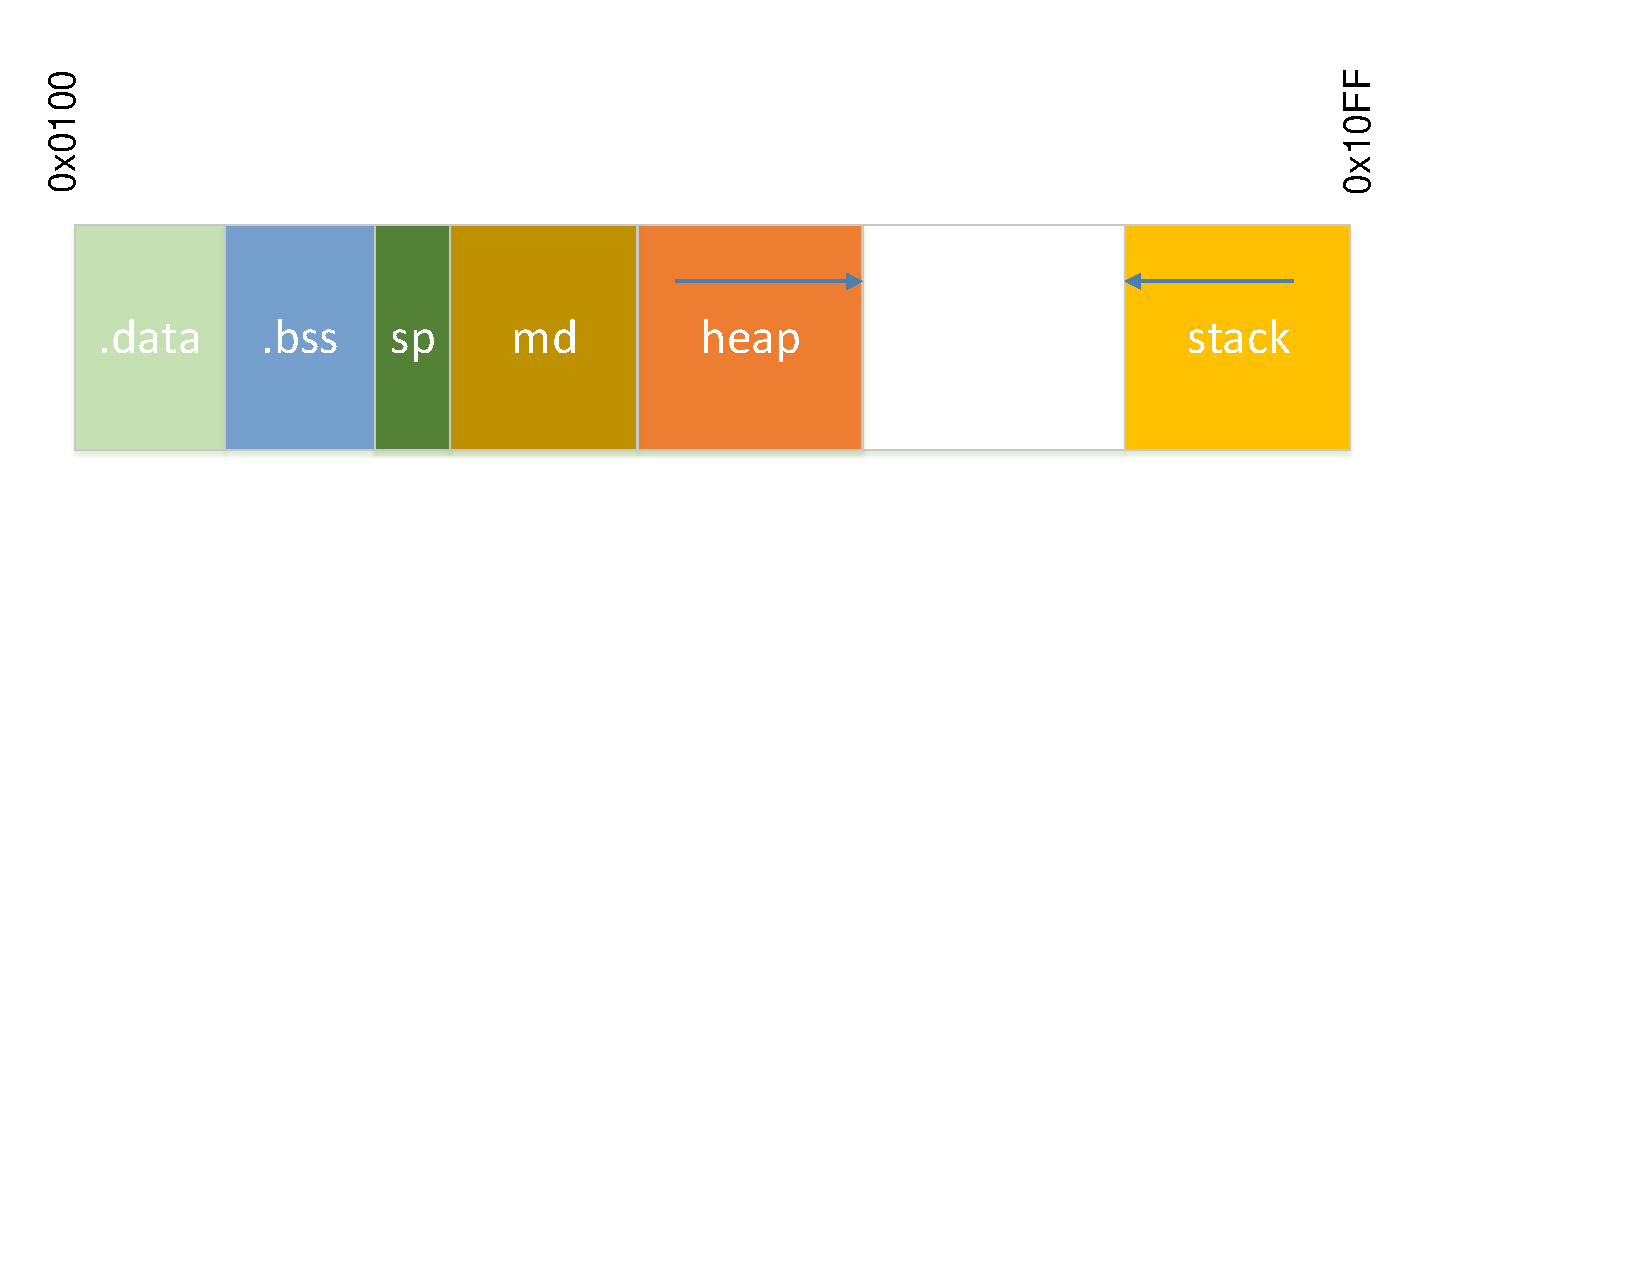
\includegraphics[scale=0.35]{figures/modified_memory_model.pdf}
\vspace{5pt}
\caption{Modified Memory Sections}
\label{fig:modified_ram_map}
\end{figure}

To store the duplicate stack frames, two new sections are created in SRAM as shown in Figure \ref{fig:modified_ram_map}, just after the \texttt{.bss} section by modifying the linker script~\cite{linkerscript}. 

The \texttt{md} section is used to store duplicate stack frames. These duplicate frames are referred to as \textit{Stack Frame Snapshots} (SFSs). The heap section grows towards the stack, and of course, the runtime usage of the heap and the stack are unpredictable. To prevent the \texttt{md} and \texttt{heap} sections from colliding, the size of the \texttt{md} section is fixed. If the heap is used, the size of the \texttt{md} section is set to 1/3 of the available space; otherwise, it is set to 1/2 of the available space. For example, if the \texttt{.data} and \texttt{.bss} sections require 1 KB in a 4 KB RAM, the space available is 3 KB, so the size of \texttt{md} is set to 1 KB.

The \texttt{sp} section is used to store the address of the next available memory space in \texttt{md}, similar to the stack pointer. This address is referred to as the \textit{Snapshot Top Pointer} (STP). To protect the STP from SEUs, the size of the \texttt{sp} section is set to 6 bytes, and 3 STP duplicates are stored in this section. Given that we assume only one SEU will occur during the execution of a given function, only one STP duplicate could be altered by a flipped bit. The altered STP is easily identified and corrected by comparing the values of the three STP duplicates.

\subsection{Injected Code Segments}

We categorize the injected code based on function. Each continuous assembly segment performs a set of operations, handling a specific action. These segments are designed to use only registers, reducing their dependency on RAM. Each segment is assigned a unique ID. Here we summarize each type of code segment.

\begin{itemize} \itemsep 0in

\item The \textit{CRC Calculation} segment (ID: CC) is used to calculate the CRC checksum of a given memory region, e.g., a stack frame. In our implementation, CRC16-CCITT is used~\cite{crc16}.

\item The \textit{CRC Save} segment (ID: CS) is used to save the CRC checksum to the stack.

\item The \textit{CRC Compare} segment (ID: CM) is used to compare two CRC checksums. The comparison result indicates whether an SEU is detected.

\item The \textit{Frame Copy} segment (ID: FC) is used to copy a stack frame to a given destination, and to save and restore stack frames.

\item The \textit{Frame Size Save} segment (ID: FS) is used to save the size of the stack frame for the current function; this will be discussed in Section \ref{sec:scanner}.

\item The \textit{STP Initialization} segment (ID: SN) is used to initialize the STP so it points to the lowest address of the \texttt{md} section.

\item The \textit{STP Update} segment (ID: SU) is used to update the STP. First, it obtains the correct STP value by comparing the three copies of the STP. Next, all three copies are updated. The segment increases the STP to save a stack frame in the SFS and decreases the STP to release a stack frame from the SFS.

\end{itemize}

\subsection{The ASM Handler}

\begin{comment}
\begin{figure*}[t]
\centering
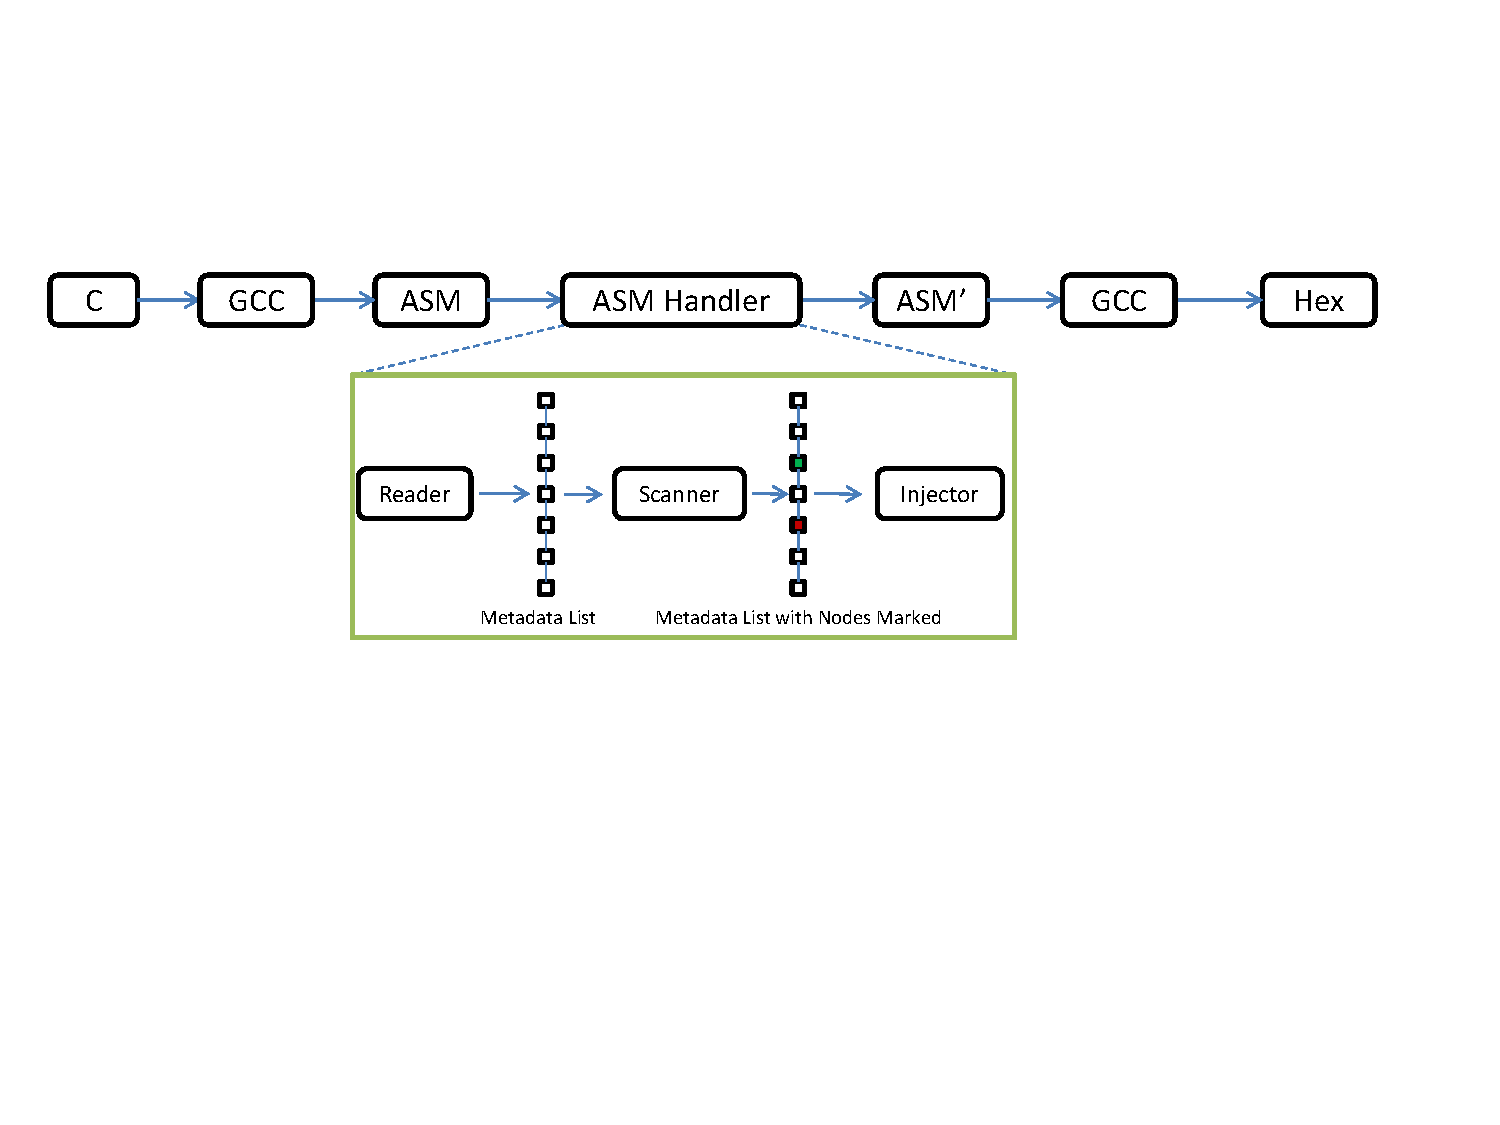
\includegraphics[width=1\textwidth]{figures/code_inject_process_v6}
\caption{Code Injection Process}
\label{fig:code_injection_process}
\end{figure*}
\end{comment}

The ASM Handler is responsible for code injection. It consists of three loosely-coupled modules: the Reader, the Scanner, and the Injector. Assembly metadata is generated to assist the code injection process. Here we describe the metadata creation process and describe each module of the ASM Handler.

\subsubsection{ASM Metadata}

Each line of assembly code is tagged with metadata representing the line of code. The metadata annotation classifies each line into one of three categories, as shown in Listing \ref{lst:metadata_example}. A \textit{directive} is used to specify assembly code information, such as the system architecture (line 1) and section (line 2), a label declaration (line 3), the label type (line 4), and other information. A \textit{label} is used to identify a location in the assembly code (line 5). In this example, \texttt{main} specifies the starting address of the main function. An \textit{instruction} is used to identify an instruction that will be executed by the microprocessor (lines 6-8). The metadata also stores code injection information, which specifies whether code is injected before or after a given line, as well as the type of code to be injected.

\begin{lstlisting}[float=tb,label=lst:metadata_example,caption=Assembly Code Example]
.arch atmega644					% directive
	.text								% directive
.global	main						% directive
	.type	main, @function		% directive
main:									% label
	push r28							% instruction
	push r29							% instruction
	...
\end{lstlisting}

\subsubsection{Reader}

The Reader is used to read the assembly file and generate corresponding metadata. It reads each line of assembly and generates a corresponding metadata node (in memory), which is then appended to a metadata list. For example, the Reader generates a list with 7 nodes after it reads the code in Listing \ref{lst:metadata_example}.%, as shown in Figure \ref{fig:code_injection_process}.

\subsubsection{Scanner}\label{sec:scanner}

The Scanner is used to scan the metadata list and mark each metadata node based on the operations performed by the associated code. Marked metadata nodes indicate that code segments will be injected either before or after the corresponding line of code.

We analyze the assembly code to identify the key operations where code segments must be injected. Here we summarize the key operations.

\begin{itemize} \itemsep 0in
\item The \textit{Stack Frame Establishment} operation is used to establish the stack frame for the current function. This operation is identified by scanning ``\texttt{sbiw r28,\textit{n}}'', which is used to establish the stack frame.

\item The \textit{Stack Frame Pointer Save} operation is used to copy the stack frame pointer to the stack pointer. This operation is identified by scanning ``\texttt{out \_\_SP\_L\_\_,r28}'', which indicates that the required registers are ready, and the function is about to execute. 

\item The \textit{Function Return} operation is used when a function returns. This operation is identified by scanning the return instruction, ``\texttt{ret}''.
\end{itemize}

The Scanner scans each node in the metadata list, checks if the code represented by the node performs one of the key operations, and marks each such node with a list of identifiers from the set (CC, CS, CM, FC, FS, SN, SU, P), where CC, CS, CM, FC, FS, SN, SU are the IDs of the code segments to be injected, and P indicates the position of the injection (i.e., before or after the assembly line). Nodes that do not require code injection are not tagged. For example, the metadata node that represents the Function Return operation is marked with (CC, CM, FC, SU, P), indicating code segments CC, CM, FC, and SU must be injected before the associated line of code.

The Scanner also extracts two information elements from the metadata list: i) The Scanner scans the metadata list and detects if \texttt{malloc} is called in the target program, which indicates whether the \texttt{heap} section in RAM is used. This information is later used in determining the section size used to store the stack frame duplicates, as discussed in Section \ref{sec:memory_sections}. ii) The Scanner determines the size of each function's stack frame by scanning the assembly code used to establish the stack frame, ``\texttt{sbiw r28, n}'', yielding a stack frame size of $n + 10$. The \texttt{n} bytes are used to store the arguments and local variables, and the additional $10$ bytes are used to store the return address, CRC, and three copies of the stack frame size, each of which requires 2 bytes.

\subsubsection{Injector}

The Injector is used to inject code segments into the target assembly code. It again scans the metadata list. When a node is marked, the Injector injects the specified code segments at the position specified by parameter $P$. Finally, a modified assembly file is generated, which is then assembled and linked to form an executable file.

In our initial approach, the code segments were directly injected into the target code, effectively making the code segments \textit{inlined}. The results showed that the ROM overhead was significant. Each function, regardless of its size, was injected with code segments that require approximately 500 bytes of ROM. In our final approach, all the code segments are injected at the end of the target code, and each is labeled with its unique ID. When scanning the metadata list, instead of injecting the code segments into the target code, a function call instruction, \texttt{call}, is injected. A function return instruction, \texttt{ret}, is added at the end of each code segment. Because each segment was designed to use only registers, only two stack bytes are needed by each segment to save the return address. We discuss the performance of both approaches in Section \ref{sec:evaluation}.

\subsection{Modified Function Execution Process}

The auxiliary code injected at the beginning and end of each function modifies the function execution process, including the invocation sub-process and the return sub-process. Below is a description of the modified processes.

\subsubsection{Modified Function Invocation Process}

The code segments injected at the beginning of each function are used to calculate a CRC over the caller's stack frame, and to save a duplicate of the caller's stack frame, as shown in Figure \ref{fig:modified_function_operation_pre_execution}. Figure \ref{fig:modified_function_operation_process_pre_execution} shows the execution process of the pre-invocation code; Figure \ref{fig:modified_function_operation_stack_pre_execution} shows the stack changes associated with the pre-invocation code. Each rectangle represents two stack bytes. In the execution process diagram, the white ovals denote operations performed by the original code, and the shaded ovals denote operations performed by the injected code. In the stack diagram, \texttt{SP} denotes the stack pointer, and \texttt{Y} denotes the stack frame pointer. As before, the numbers below each stack identify the operations that changed the stack.

When a function \texttt{B} is called by a function \texttt{A}, the return address is pushed onto the stack automatically by the function call instruction (step 1). To calculate the CRC of the caller's stack frame, multiple registers are used, so they must be saved before the CRC calculation process, and restored when the process is finished. To prevent the calculated CRC from being overwritten when the registers are restored, two bytes are pushed onto the stack as a placeholder (step 2) for the CRC result before the registers used to calculate the CRC are saved (step 3). After the CRC of function \texttt{A}'s stack frame is calculated (step 4), the CRC result is saved to the placeholder location (step 5). The registers used to calculate the CRC are then restored (step 6).

Next, the stack frame of the caller, function \texttt{A}, has to be saved. The registers used to save the stack frame are pushed onto the stack (step 7). Next, the correct STP is selected by comparing the values of the three STP copies (step 8). Using the correct STP, the specified memory is then copied and saved in the SFS (step 9). After the STP copies are updated (step 10), the CRC registers are restored (step 11).

After the stack frame pointer of function \texttt{B} is saved (step 12), and the stack frame is established (step 13), three copies of the stack frame size of the callee, function \texttt{B}, are pushed onto the stack (step 14), which is a key operation in the injected code. 

When a function is called, the return address is pushed onto the stack, and later used when the function returns. However, the callee does not have sufficient context regarding its caller, including the caller's stack frame address and size. It is impossible for the callee to calculate the CRC of the caller's stack frame and to duplicate the stack frame without this information. To solve this problem, each function saves its stack frame size in the stack, which is used by its callee to perform the CRC calculation and stack frame copy. To ensure the correctness of the stack frame size, three copies are saved. Comparison is used to yield the correct value. 

\begin{figure}[h]
        \centering
        \begin{subfigure}[b]{0.4\columnwidth}
                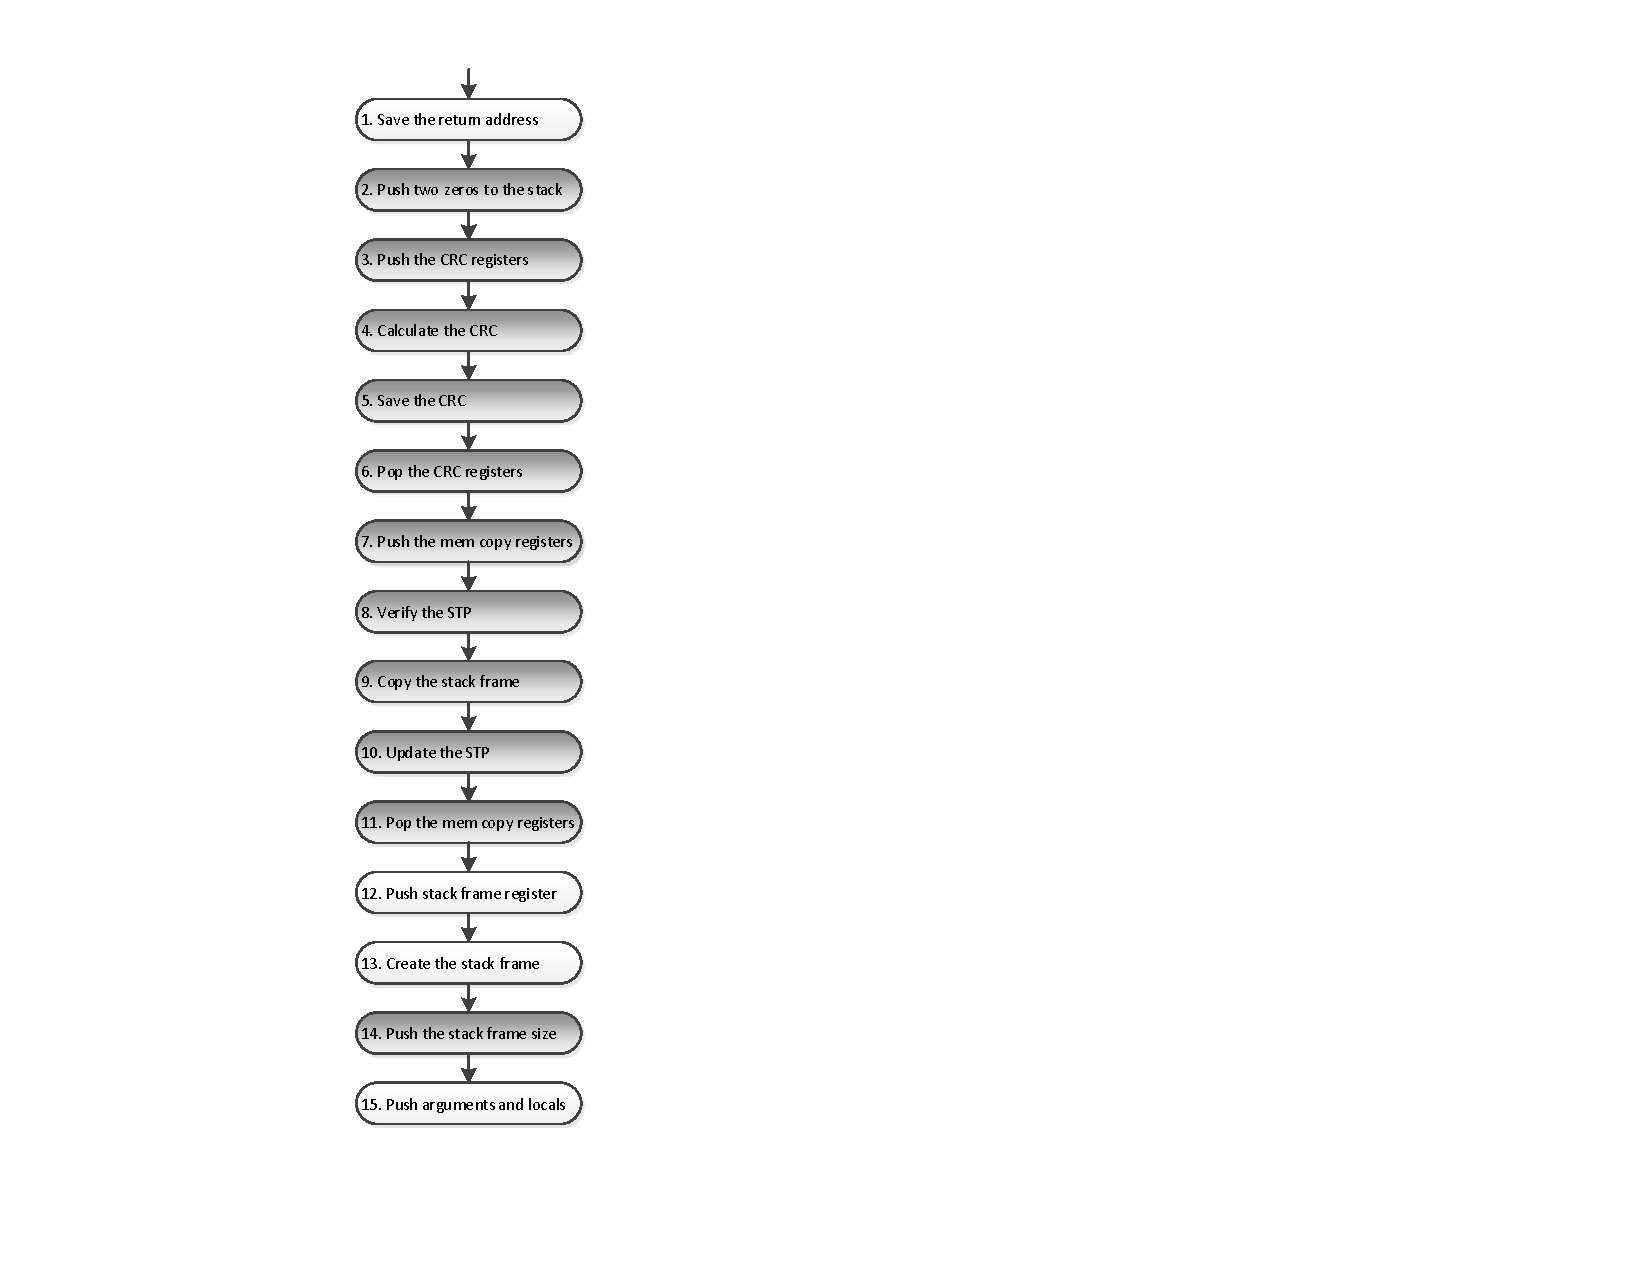
\includegraphics[width=\textwidth, height=12cm]{figures/modified_function_operations_process_pre_execution_v2}
                \caption{Process}
                \label{fig:modified_function_operation_process_pre_execution}
        \end{subfigure}~
        \begin{subfigure}[b]{0.6\columnwidth}
                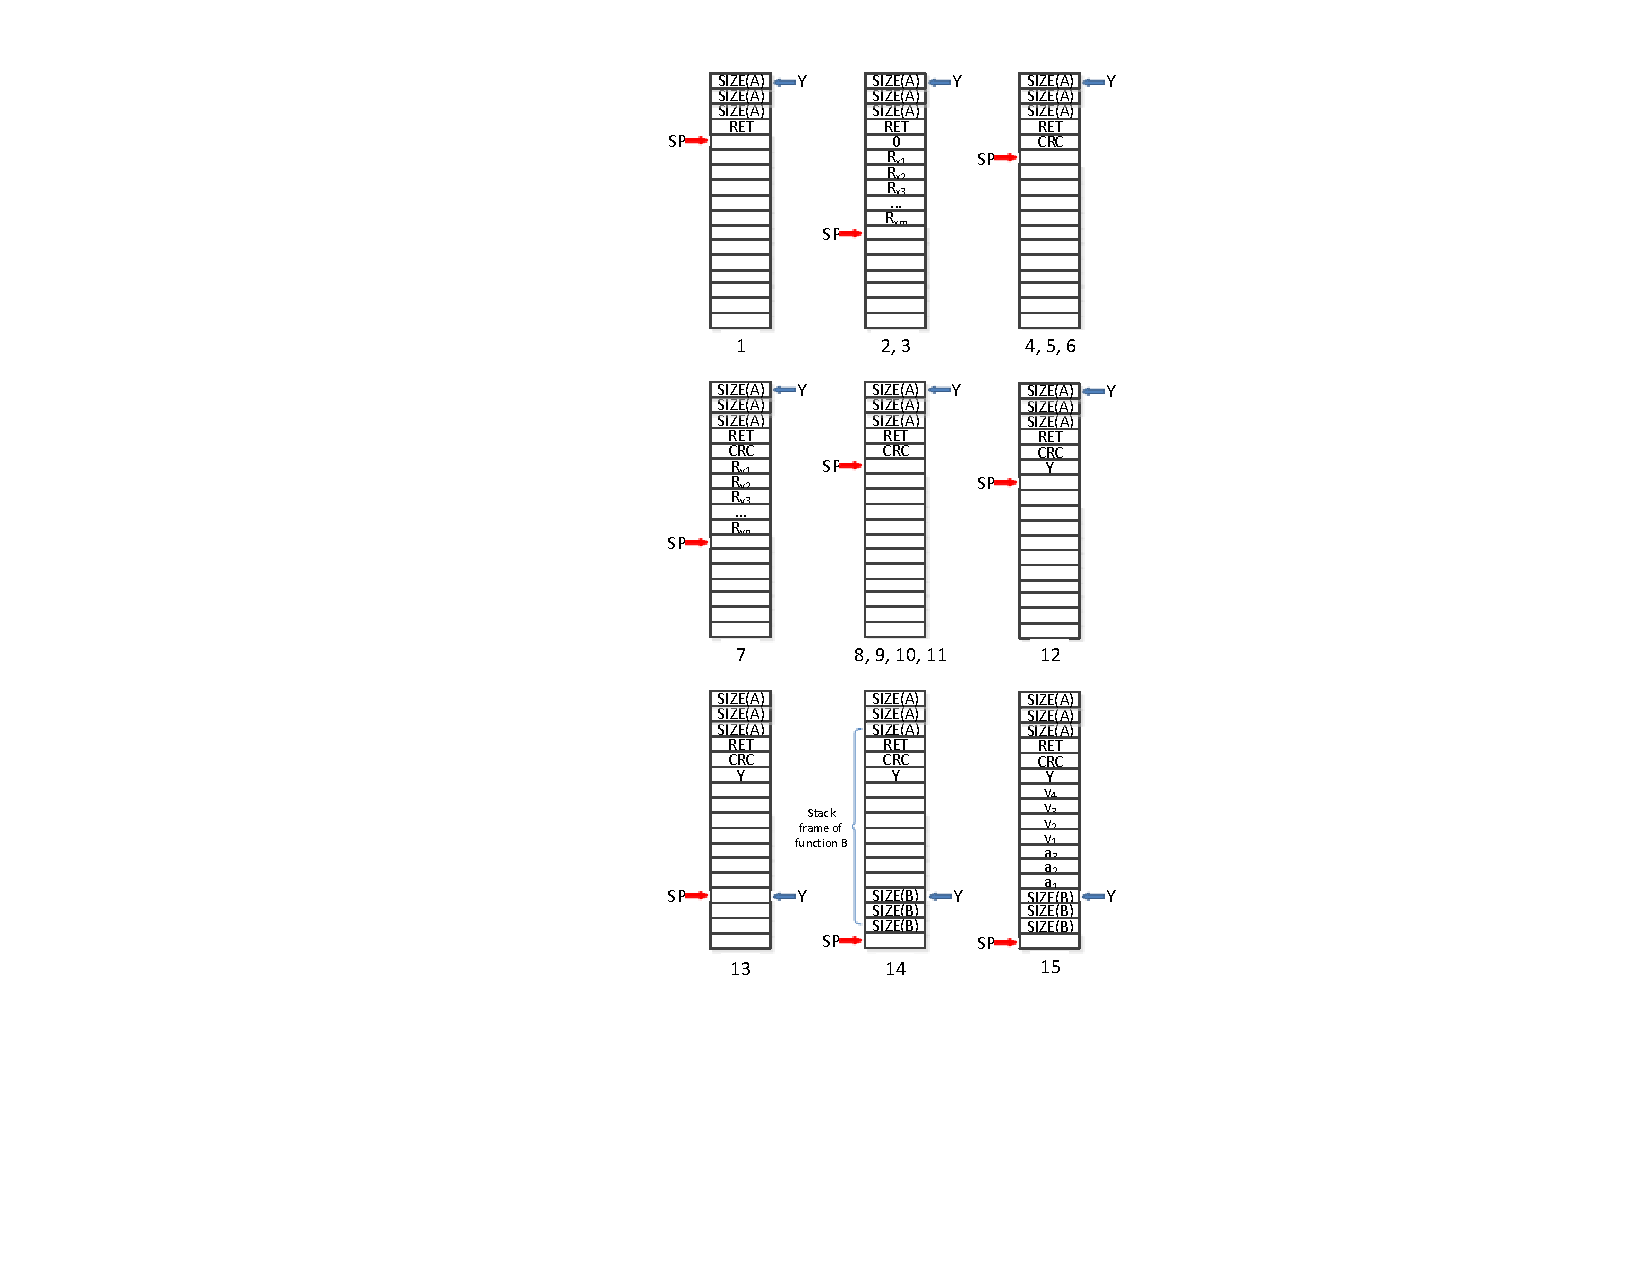
\includegraphics[width=\textwidth, height=12cm]{figures/modified_function_operations_stack_pre_execution_v2}
                \caption{Stack}
                \label{fig:modified_function_operation_stack_pre_execution}
        \end{subfigure}
		\vspace{10pt}
        \caption{Modified Function Invocation Process}\label{fig:modified_function_operation_pre_execution}
\end{figure}

\subsubsection{Modified Function Return Process}

The code segments injected at the end of each function are used to verify the stack frame of the caller function, and to restore the stack frame if an SEU is detected, as shown in Figure \ref{fig:modified_function_operation_post_execution}. Each rectangle represents two stack bytes. Again, in the execution process diagram, the white ovals denote operations performed by the original code, and the shaded ovals denote operations performed by the injected code.

When function \texttt{B} returns, it first pops its stack frame size (step 1). After the space used to store the arguments and local variables is released (step 2), the stack frame pointer is restored (step 3). The CRC of function \texttt{A}'s stack frame is then calculated and temporarily stored in two registers (steps 4-6). The values stored in these registers are saved before the function return process. Next, the calculated CRC is compared with the CRC saved in the stack (step 7). If the two CRCs do not match, the saved stack frame of \texttt{A} is restored, and the STP is updated to release the space used to store the stack frame of \texttt{A} (steps 8-12). Again, the stack frame size of function \texttt{A} saved in the stack is used to support the CRC comparison and stack frame restoration (if needed). If the two CRCs match, the STP is updated (steps 13-14). After verification of \texttt{A}'s stack frame is complete, the CRC is popped from the stack (step 15). Finally, function \texttt{B} returns, and the return address is popped automatically (step 16).

\begin{figure}[h]
        \centering
        \begin{subfigure}[b]{0.5\columnwidth}
                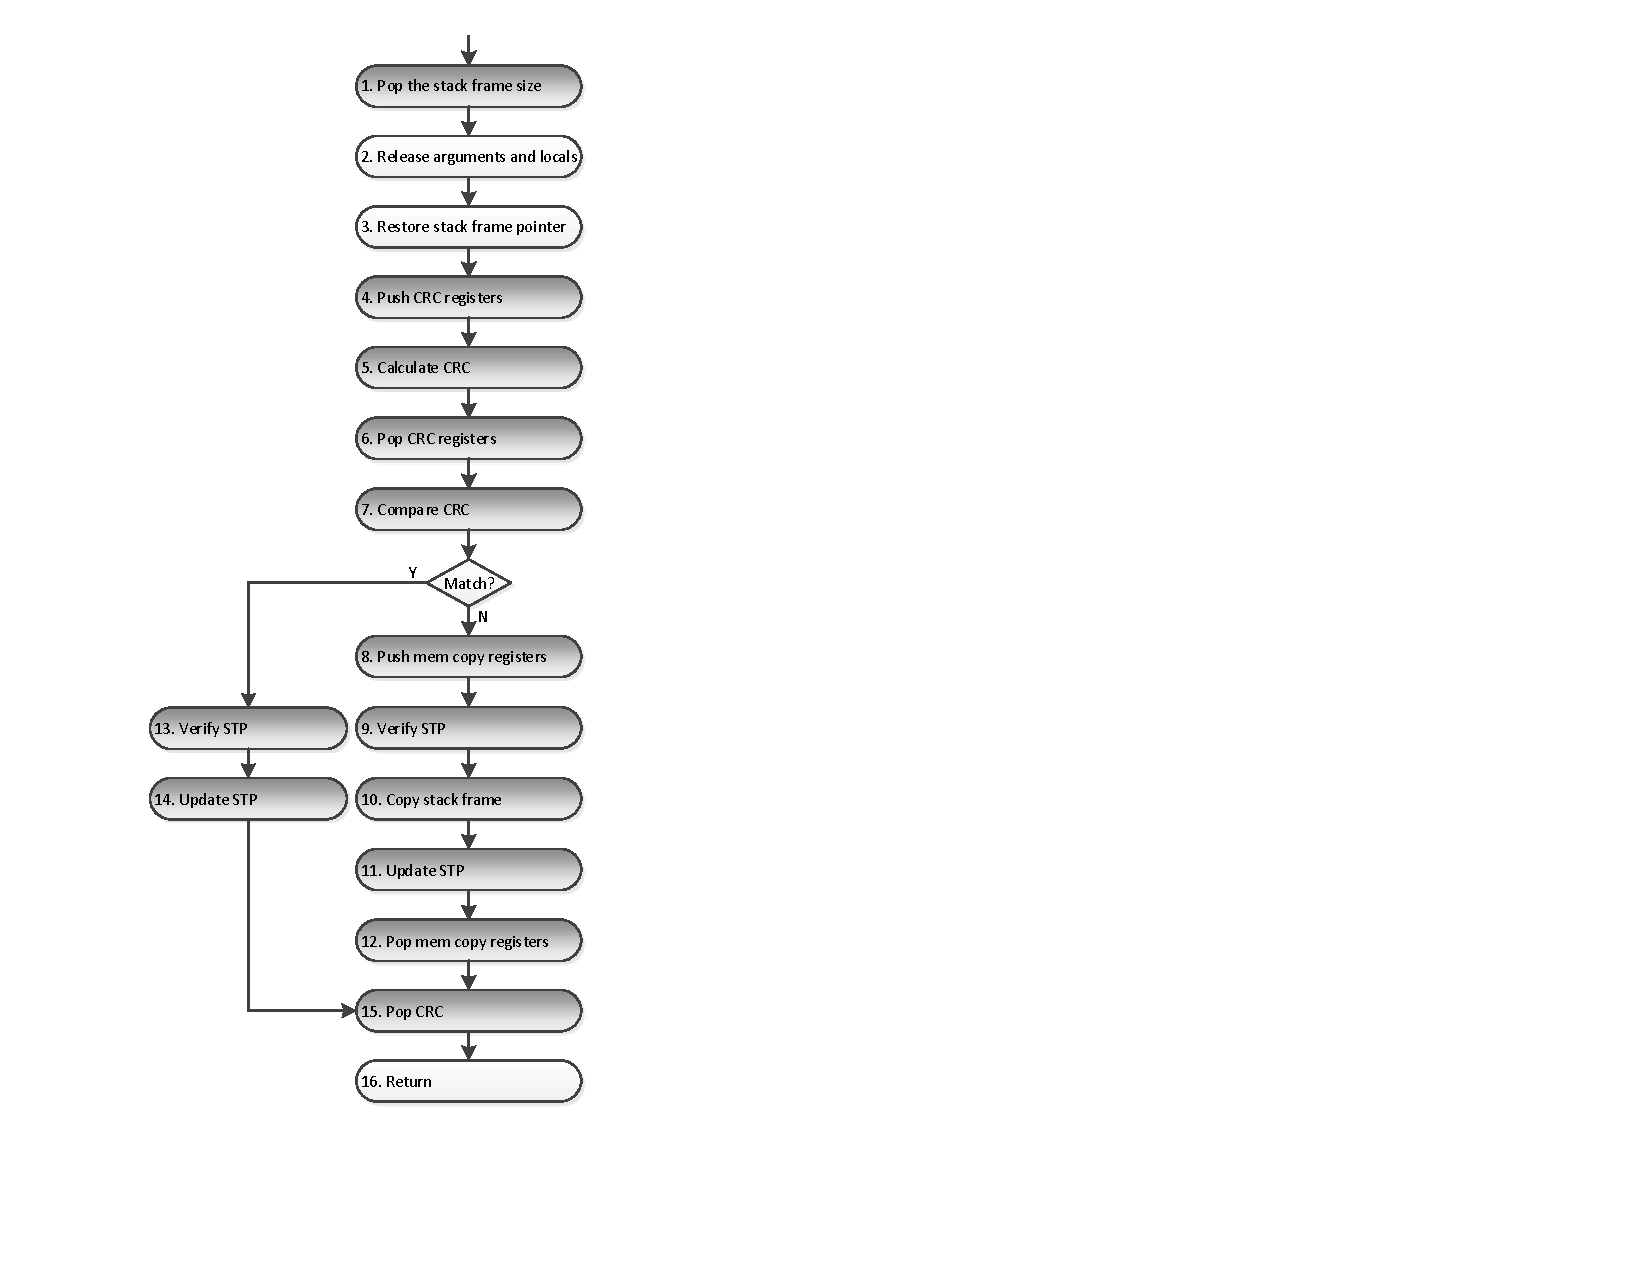
\includegraphics[width=\textwidth, height=12cm]{figures/modified_function_operations_process_post_execution_v2}
                \caption{Process}
                \label{fig:modified_function_operation_process_post_execution}
        \end{subfigure}~
        \begin{subfigure}[b]{0.5\columnwidth}
                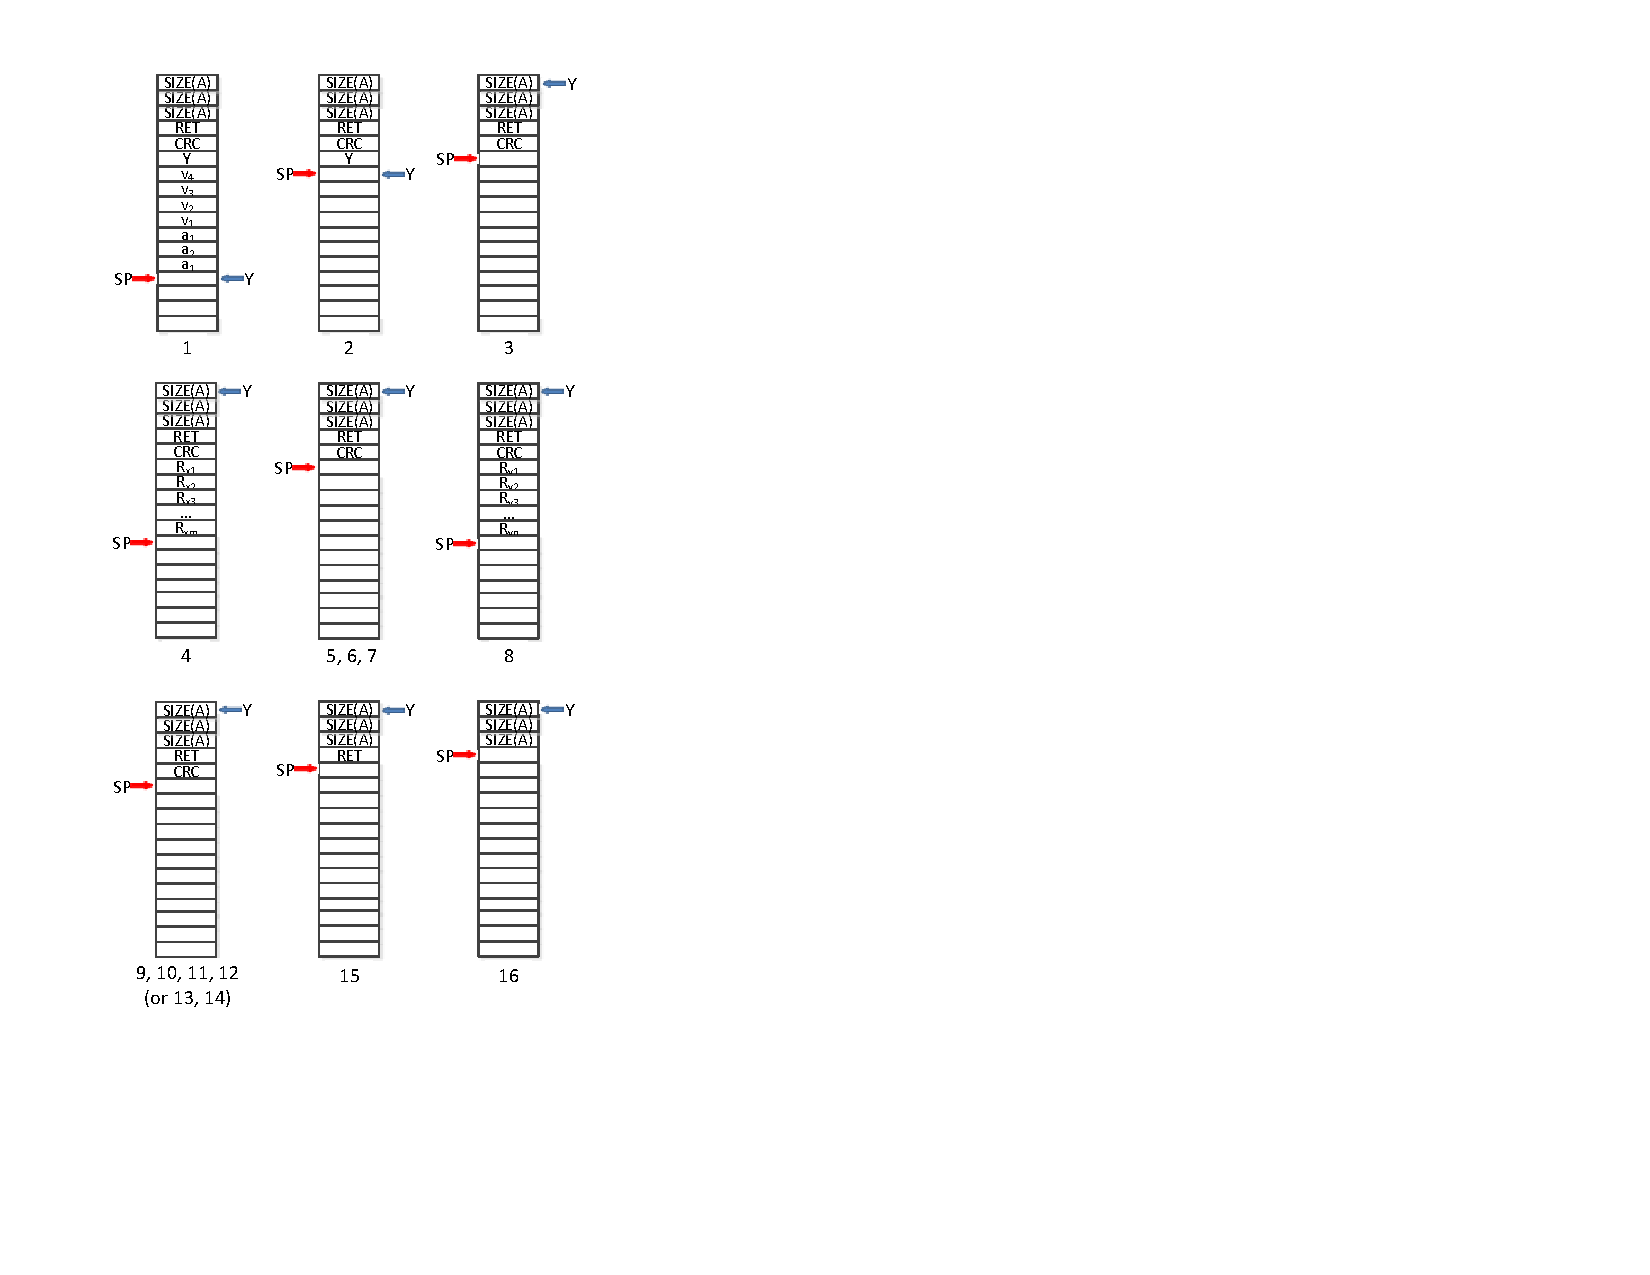
\includegraphics[width=\textwidth, height=12cm]{figures/modified_function_operations_stack_post_execution_v2}
                \caption{Stack}
                \label{fig:modified_function_operation_stack_post_execution}
        \end{subfigure}
        \vspace{10pt}
        \caption{Modified Function Return Process}\label{fig:modified_function_operation_post_execution}
\end{figure}

\section{Evaluation}\label{sec:evaluation}

Here we present our evaluation of the SEU protection approach. We first introduce three test applications with different degrees of stack dynamism. We then validate the correctness of our approach and analyze the relationship between protection efficacy and the SEU injection rate. Finally, we consider the overhead introduced by our approach, both in terms of space and execution speed. Ubuntu 13.10, with Linux kernel version 3.8, and GCC 4.1.2 are used.

\subsection{Test Applications}

To evaluate our approach under varying stack conditions and SEU injection rates, three AVR applications are considered. The stack usage pattern of each application is shown in Figure \ref{fig:stacksize_usage}. The x-axis represents execution time, and the y-axis represents stack size. Below is a description of each application.

\begin{itemize}
\item The \textbf{Delay} application repeatedly executes a function that contains a delay of 2,040 clock cycles, implemented using a while loop, yielding low stack variability.
\item The \textbf{Double Function Calls} application repeatedly executes three functions --- function A calls B, and function B calls C --- yielding moderate stack variability.
\item The \textbf{Fibonacci} application repeatedly calculates the tenth Fibonacci number using recursion, yielding significant stack variability.
\end{itemize}

\begin{figure}[h]
\centering
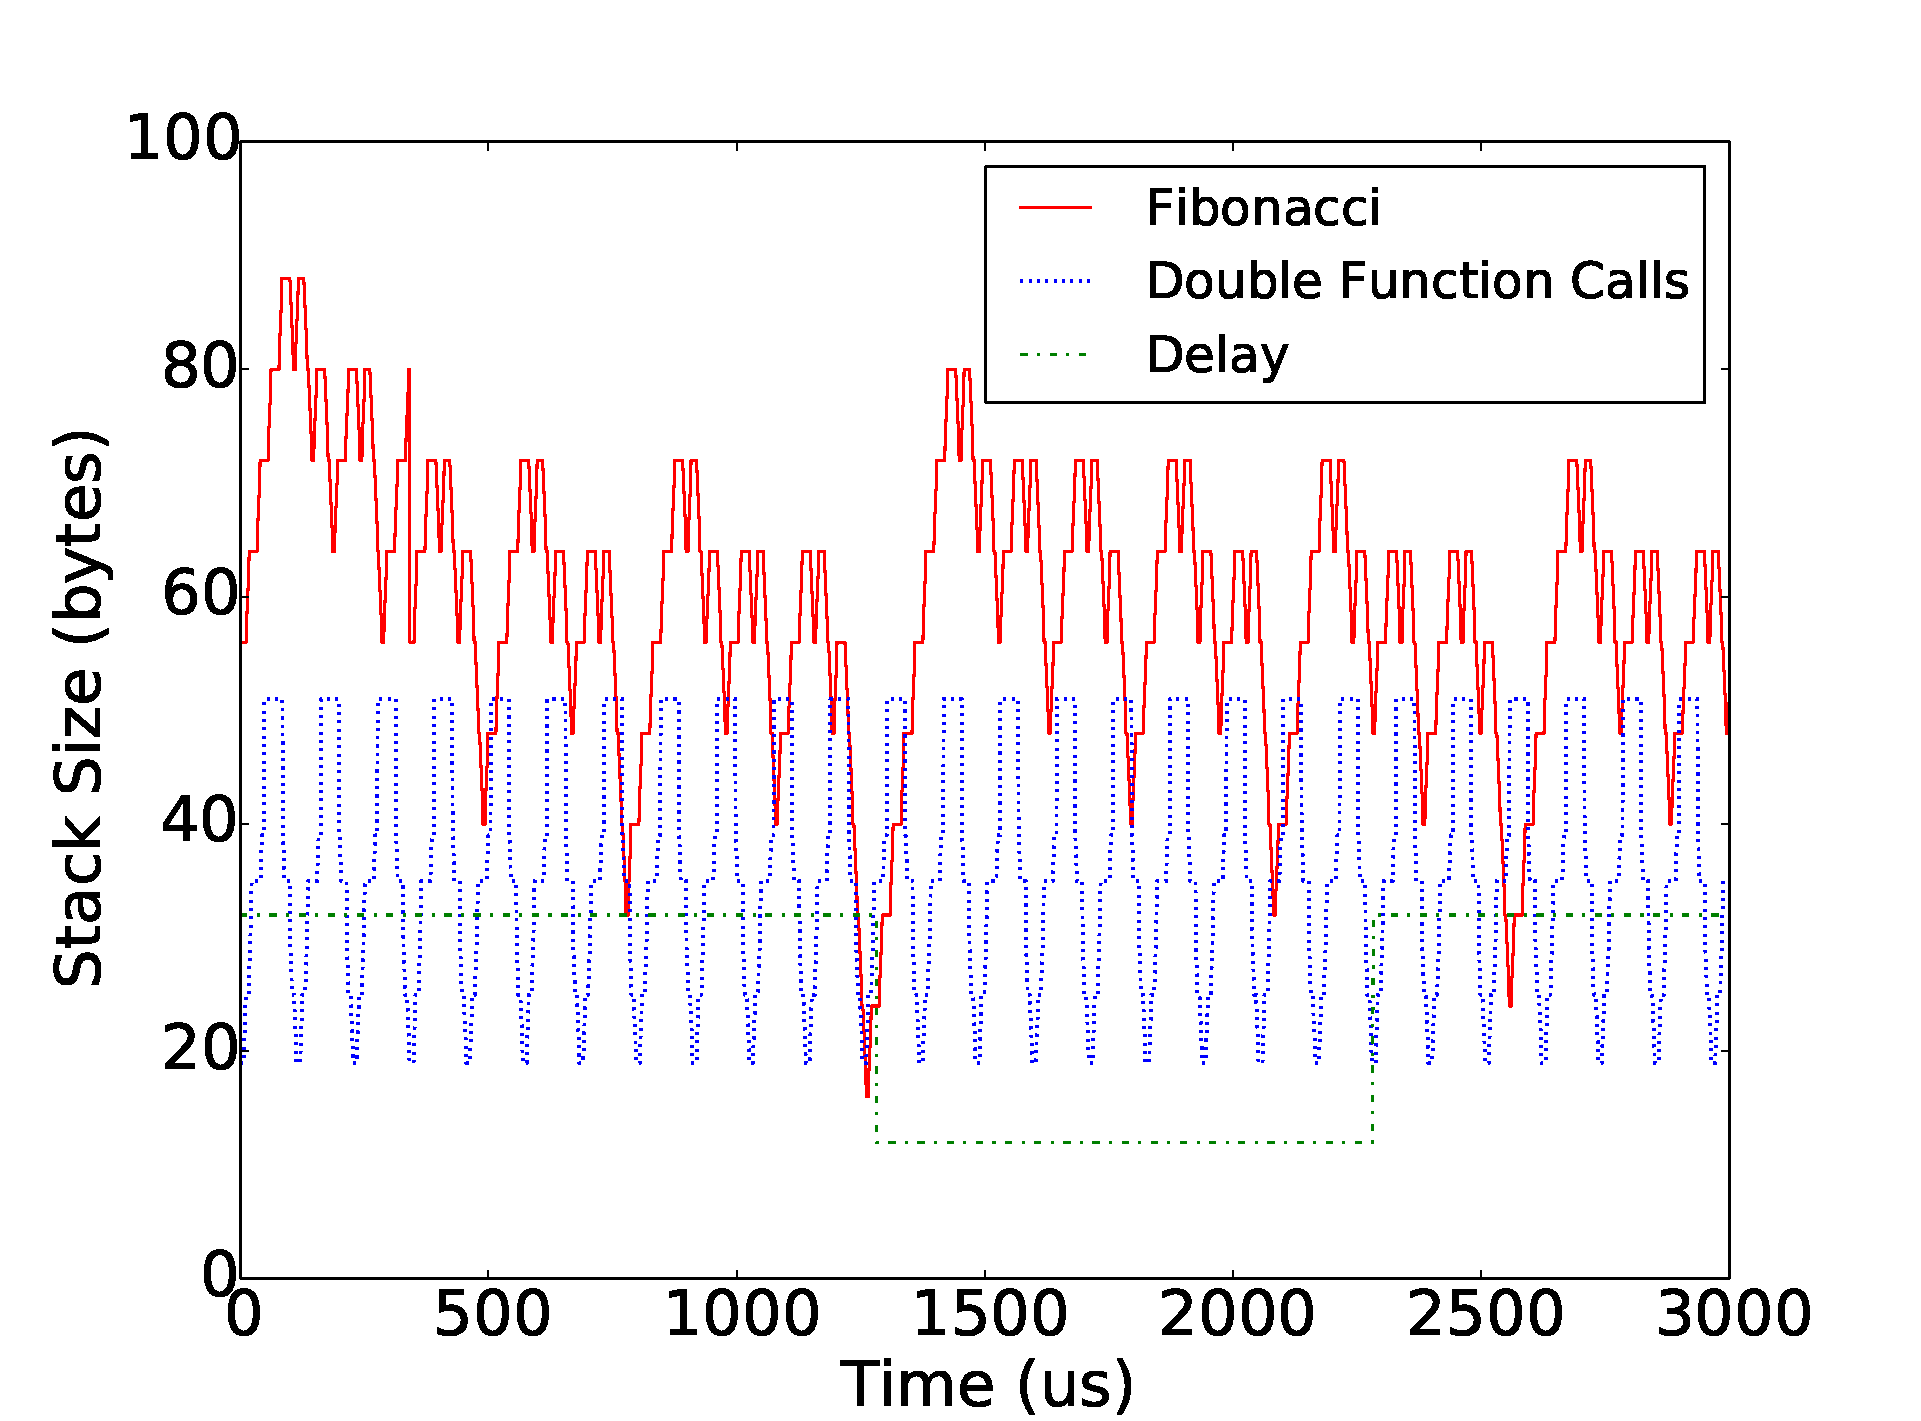
\includegraphics[width=0.48\textwidth]{figures/stacksize_usage_v3.pdf}
\vspace{5pt}
\caption{Stack Usage of Test Applications}
\label{fig:stacksize_usage}
\end{figure}

\subsection{Validation}

We first validate our approach and consider the SEU protection efficacy it affords. Recall the modified SRAM partition shown in Figure \ref{fig:modified_ram_map}. In our analysis, we ignore both the .data and the .bss sections, as well as the heap section. Data stored in the .data, .bss, and heap sections can be protected using well-known techniques based on cloning and comparison. We focus our analysis on stack frame protection. Again, the injected code segments used to protect the stack frames are designed to use only registers, and each segment requires only two bytes in the currently executing function's stack frame (for the return address).
%A embedded application is typically designed based on interrupts, and usually contains an infinite loop in a function, which never returns. If the function which has the infinite loop is not the \textit{main} function (although it is the \textit{main} function for most times), the stack frame of the function's caller is not protected. However, since the stack space containing the function and its callers' stack frames doesn't change during the execution of the applications, the space can be identified using static analysis and can be protected using cloning and comparison. This issue will be addressed in our future work.

We first assume that the currently executing function's frame, which includes the return address of the injected code segment, is not affected by SEUs. We use induction to prove the correctness of our approach. Suppose \textit{n} is the number of stack frames stored in the stack, excluding the frame for \textit{main}.

\textbf{Base Case:} If $n=0$, only the stack frame of \textit{main} is on the stack. When \textit{main} calls another function, say \textit{foo}, the stack frame for \textit{foo} is created. According to our assumption, the current stack frame (\textit{foo}'s) will not be affected by SEUs during execution. When \textit{foo} returns, the stack frame of \textit{main} is protected by our approach. So the stack frames of caller and callee are guaranteed to be correct if any function is invoked and returns when $n=0$.

\textbf{Induction Assumption:} Assume that the stack frames of callers and callees are guaranteed to be correct for $n=k$, where $k\geq 1$.

\textbf{Inductive Step:} Now consider $n=k+1$. Assume \textit{a} is the current function, which calls \textit{b}. According to our assumption, b's stack frame is not affected by SEUs. When \textit{b} returns, the stack frame of \textit{a} is protected by our approach. So the stack frames of callers and callees are guaranteed to be correct when $n=k+1$. The currently executing function's stack frame is assumed safe, and the stack frames of callers and callees are protected against SEUs during execution; by induction, the stack is guaranteed to be correct, assuming the current stack frame is never affected by SEUs.

To verify this claim, the AVR Simulator IDE~\cite{avrsimide} was used to manually inject SEUs, and to observe execution results. The results showed that each function is able to detect and fix SEUs introduced ``beneath'' the topmost stack frame.

However, if the stack frame of the current function is affected by an SEU, protection is not guaranteed. If the SEU changes key data, such as the return address or stack frame size, the current function will not execute as expected. We assume that only one SEU will occur during a given function execution, and that the SEU is uniformly likely to affect all bits in RAM. The probability of successful SEU protection can be expressed as:
\begin{equation}\label{eq_seu1}
p=1-\frac{c}{2s+e-c+6}
\end{equation}
Where $p$ is the probability of successful protection, $s$ is the stack size, $e$ is the size of the unused space in RAM, $6$ is the size of the three STP copies, and $c$ is the average size of a stack frame. Since the return address of the injected code segment is stored in the current stack frame, the two bytes for the return address are included in c. The total size of protected memory is $s+e+(s-c)+6$, where $s-c$ is the size of the stack frame copies stored in the \textit{md} section.

We extend our analysis to cases where more than one SEU may occur during a given function execution. Our approach succeeds when the following conditions are met: (i) the currently executing function's stack frame is not affected (so the return address of the injected code segment is not affected); (ii) at least two of the three copies of the caller's stack frame size are not affected; (iii) at least two of the three copies of the STPs are not affected; and (iv) at least one of the two caller's stack frames (the original and the backup copy saved in the \texttt{md} section) is not affected. To simplify the analysis, conditions (ii) and (iii) are strengthened, requiring that all three copies of the caller's stack frame size cannot be affected, and all three copies of the STPs cannot be affected. Since the strengthened conditions slightly reduce the probability of successful SEU protection (only 4 bytes are ignored), the real probability of protection is slightly higher than the presented results. The probability of successful SEU protection can be expressed as:
\begin{equation}\label{eq_seu2}
\begin{split}
&p=(1-\frac{c}{2s+e-c+6})^n*(1-\frac{6}{2s+e-2c+6})^n \\
&*(1-\frac{6}{2s+e-2c})^n*\{(1-\frac{2c}{2s+e-2c-6})^n \\
&+ \mathrm{C}_2^1*(1-\frac{c}{2s+e-2c-6})^n\\
&*[1-(1-\frac{c}{2s+e-3c-6})^n]\}
\end{split}
\end{equation}

Where $p$ is the probability of success, $s$ is the size of the stack, $e$ is the size of the unused space in RAM, $6$ is the size of the three stack frame size copies or the three STP copies, $c$ is the average size of the stack frame (including the return address of the injected code segment), and $n$ is the number of SEUs that occur during a function's execution. In equation \ref{eq_seu2}, $(1-\frac{c}{2s+e-c+6})^n$ is the probability that the currently executing function's stack frame is not affected by SEUs. $(1-\frac{6}{2s+e-2c+6})^n*(1-\frac{6}{2s+e-2c})^n$ is the probability that both copies of the caller's stack frame size and the three STPs are not affected by SEUs. Within the curly brackets, $(1-\frac{2c}{2s+e-2c-6})^n$ is the probability that both the original and the copy of the caller's stack frame are not affected by SEUs. $\mathrm{C}_2^1*(1-\frac{c}{2s+e-2c-6})^n*[1-(1-\frac{c}{2s+e-3c-6})^n]$ is the probability that either the original or the copy of the caller's stack frame is affected by SEUs. So $\{(1-\frac{2c}{2s+e-2c-6})^n + \mathrm{C}_2^1*(1-\frac{c}{2s+e-2c-6})^n*[1-(1-\frac{c}{2s+e-3c-6})^n]\}$ is the probability that at least one --- the original or the copy --- of the caller's stack frames is not affected.

In equation \ref{eq_seu2}, the number of SEUs that occur, $n$, can be expressed as:
\begin{equation}
n = \frac{y*l}{m}*f
\end{equation}
where $y$ is the number of clock cycles used to execute each instruction, $m$ is the frequency of the microprocessor, $l$ is the average number of function instructions, and $f$ is the SEU injection rate. Most AVR instructions require 2 clock cycles to execute, and the frequency of our ATmega644 is set to 10MHz.

\begin{table}
	\center
    \begin{tabular}{|l|c|c|c|c|}
    \hline
    \textbf{Applications}   & \textbf{l} & \textbf{c} & \textbf{s} & \textbf{e}	\\ \hline
    Fibonacci             		& 42			& 10		& 60	   	& 2992		\\
\hline
    Double Function Calls       & 54			& 9			& 30        & 3022		\\ \hline
    Delay         				& 115			& 16		& 30		& 3022		\\
 \hline
    \end{tabular}
    \vspace{5pt}
    \caption {Application Characteristics}
    \label{tbl_application_parameters}
\end{table}
\begin{figure}
\centering
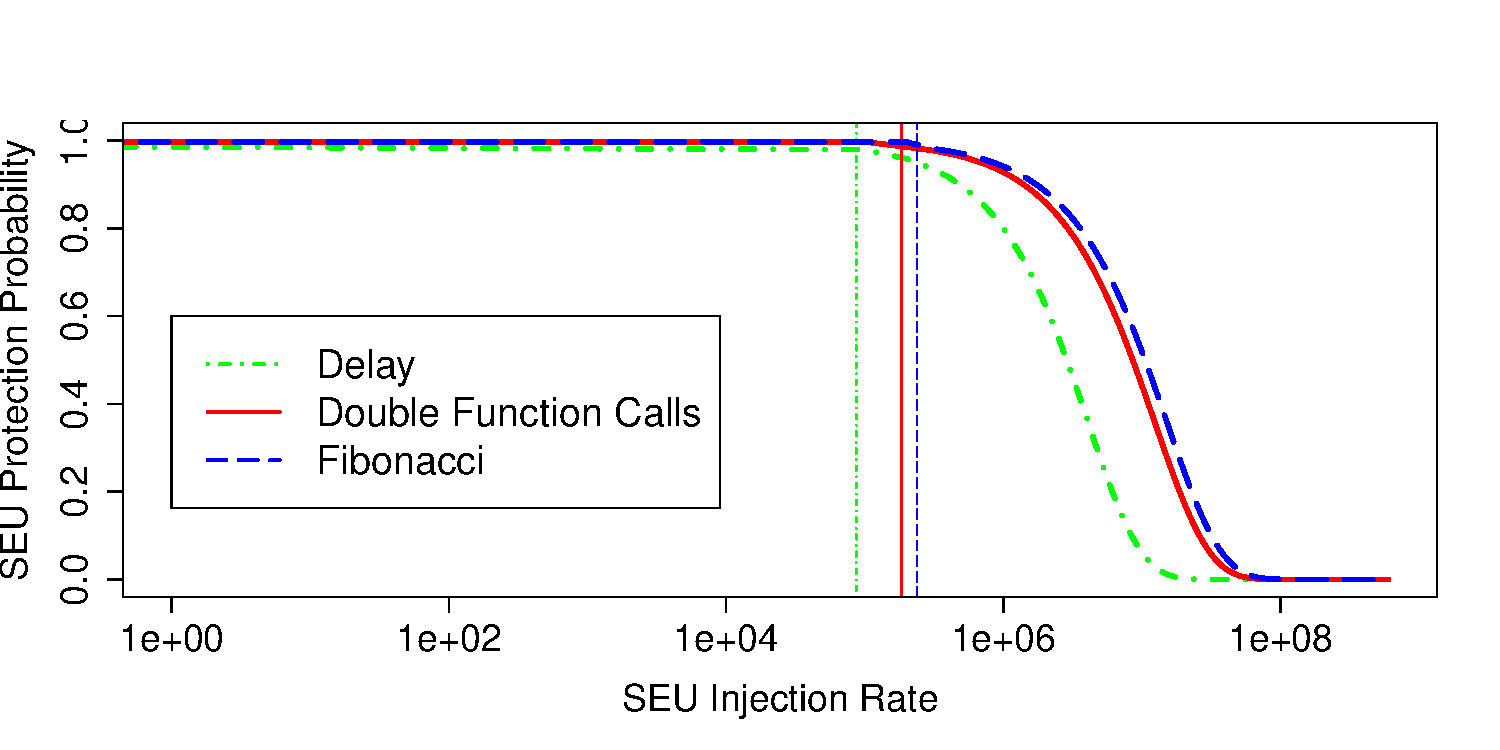
\includegraphics[width=0.48\textwidth, height=130pt]{figures/success_probability_v2.pdf}
\vspace{5pt}
\caption{SEU Protection Probability}
\label{fig:success_probability}
\end{figure}
We now consider the relationship between SEU protection probability and SEU occurrence rate. To demonstrate the relationship, we collect the corresponding parameters for the three test applications using AVR Simulator IDE, as shown in Table \ref{tbl_application_parameters}. Figure \ref{fig:success_probability} plots the change in SEU protection probability as a function of SEU injection rate. The x-axis represents the rate at which SEUs are injected, and the y-axis represents the corresponding SEU protection probability. Each vertical line marks where the number of SEUs begins to exceed 1 (for each application). When only one SEU occurs during a given function execution (left side of the vertical line), the SEU protection probability is constant (Delay: 99.48\%, Double Function Calls: 99.71\%, Fibonacci: 99.68\%) because the only case the approach cannot handle is when the current frame is affected. When more than one SEU occurs during a given function execution (right side of the vertical line), the SEU protection probability increases because the SEUs may affect the stack frame of the current function, the stack frame sizes of the caller stored in the stack, the STPs, and stack frame copies stored in the \texttt{md} section. As the SEU occurrence rate increases, the SEU protection probability decreases, until it approaches 0. The lower the stack dynamism, the longer the function execution time, which increases the probability of SEU occurrence in the current stack frame. Low stack frame dynamism causes the SEU protection probability for Delay to drop significantly compared to the other applications.

\subsection{Performance}

Since the same code is injected for every function, the execution overhead is similar for all functions, varying only when an SEU is detected. Table \ref{tbl_speed_overhead} summarizes the overhead of each injected code segment. The second column lists the number of times each code segment executes (per function execution), the third column lists the number of instructions executed in each code segment, the fourth column lists the number of clock cycles spent executing each code segment, and the fifth column lists the ROM space overhead for each injected segment. $S$ denotes the size of the (recovered) stack frame. The \textit{CRC calculation} code segment and \textit{STP update} code segment execute twice for each function, and the \textit{frame copy} code segment executes either once or twice, depending on whether an SEU is detected. Each of the other code segments executes once for each function execution. Therefore, the minimum overhead introduced in terms of number of clock cycles is $62*S+304$, when an SEU is not detected. The worst case is $70*S+432$ clock cycles, when an SEU is detected. 
\begin{table*}
	\center
    \begin{tabular}{|l|c|c|c|c|}
    \hline
   \textbf{Code Segment}   & \textbf{Number of Execution} & \textbf{Instructions} & \textbf{Clock Cycles} & \textbf{ROM Space}	\\ \hline
    CRC Calculation         & 2			& 24*S+1		& 27*S+4		& 50				\\ \hline
    CRC Save                & 1			& 13			& 26           	& 26				\\ \hline
    CRC Compare             & 1			& 27			& 52		   	& 64				\\ \hline
    Frame Copy				& 1 or 2	& 64+4*S		& 8*S+128      	& 50				\\ \hline
%    Frame Copy (Worst Case) & 1 		& 73+4*S      & 144+8*S      & 50				\\ \hline
    Frame Size save         & 1			& 18			& 34           	& 36				\\ \hline
    STP Initialization		& 1			& 16			& 28		   	& 32				\\ \hline
	STP Update				& 2			& 7				& 14			& 14				\\ \hline
	\textbf{Total (No Recovery)} & -	 	& 48*S+154     	& 62*S+304		& 272  		\\ \hline
	\textbf{Total (Recovery)}& -	 		& 52*S+218     	& 70*S+432		& 272 		\\ \hline
    \end{tabular}
	\vspace{5pt}
    \caption {Execution Overhead}
    \label{tbl_speed_overhead}
\end{table*}

We next evaluate space overhead using the three test applications. The ROM space data was collected using \textit{avr-size}. The results are summarized in Figure \ref{fig:space_overhead}. The y-axis represents ROM size, in bytes. Delay and Fibonacci involve two functions, and Double Function Calls involves four. From Figure \ref{fig:space_overhead}, we can see that the ROM overhead for the Double Function Calls application is twice the Delay and Fibonacci applications. ROM overhead is related only to the number of functions in the program.

\begin{figure}[h]
\centering
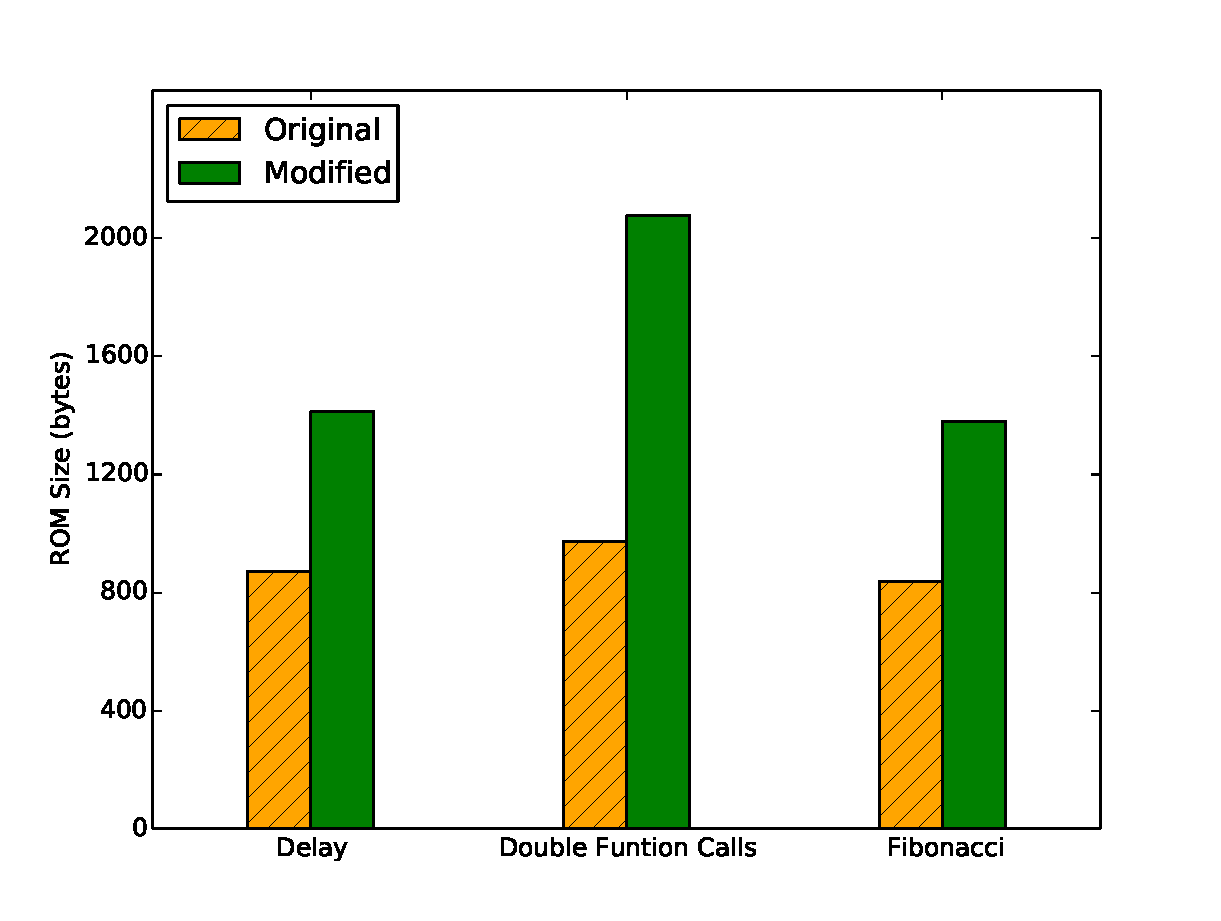
\includegraphics[scale=0.47]{figures/space_overhead.pdf}
\caption{ROM Overhead}
\vspace{5pt}
\label{fig:space_overhead}
\end{figure}

We next evaluate execution overhead. As shown in Table \ref{tbl_speed_overhead}, the execution overhead for every function call is determined by the size of the stack frame. We consider the execution overhead as a function of the average number of instructions executed between each call instruction (i.e., an inverse measure of call frequency). The execution overhead can be expressed as:
\begin{equation}\label{eq_seu1}
e=\frac{l+L}{l}
\end{equation}
Where \textit{L} is the number of injected machine instructions for each function, and \textit{l} is the average number of machine instructions executed between each call instruction. As summarized in Table \ref{tbl_speed_overhead}, $L=48*S+154$ when no SEUs are detected, and $L=52*S+218$ when an SEU is detected. The average frame size, $S$, is 20. The overhead results are summarized in Figure \ref{fig:speed_overhead}. The x-axis represents the average number of instructions executed between function invocations (\textit{l}), and the y-axis represents execution overhead, measured as the ratio between the execution speed of the original code and the modified code. The figure shows that given the same stack frame size, execution overhead is determined by stack dynamism. The less stack dynamism, the less speed overhead. The explanation is that within a given period of time, increased function calls lead to increased execution of the injected code. The results reveal an interesting tradeoff among dynamism, protection efficacy, and performance. Increasing dynamism offers better protection, but worse performance; decreasing dynamism offers better performance, but less protection. Knowledge of this tradeoff can be used to inform the function decomposition process, enabling embedded designers to appropriately balance protection efficacy and execution overhead.
\begin{figure}
\centering
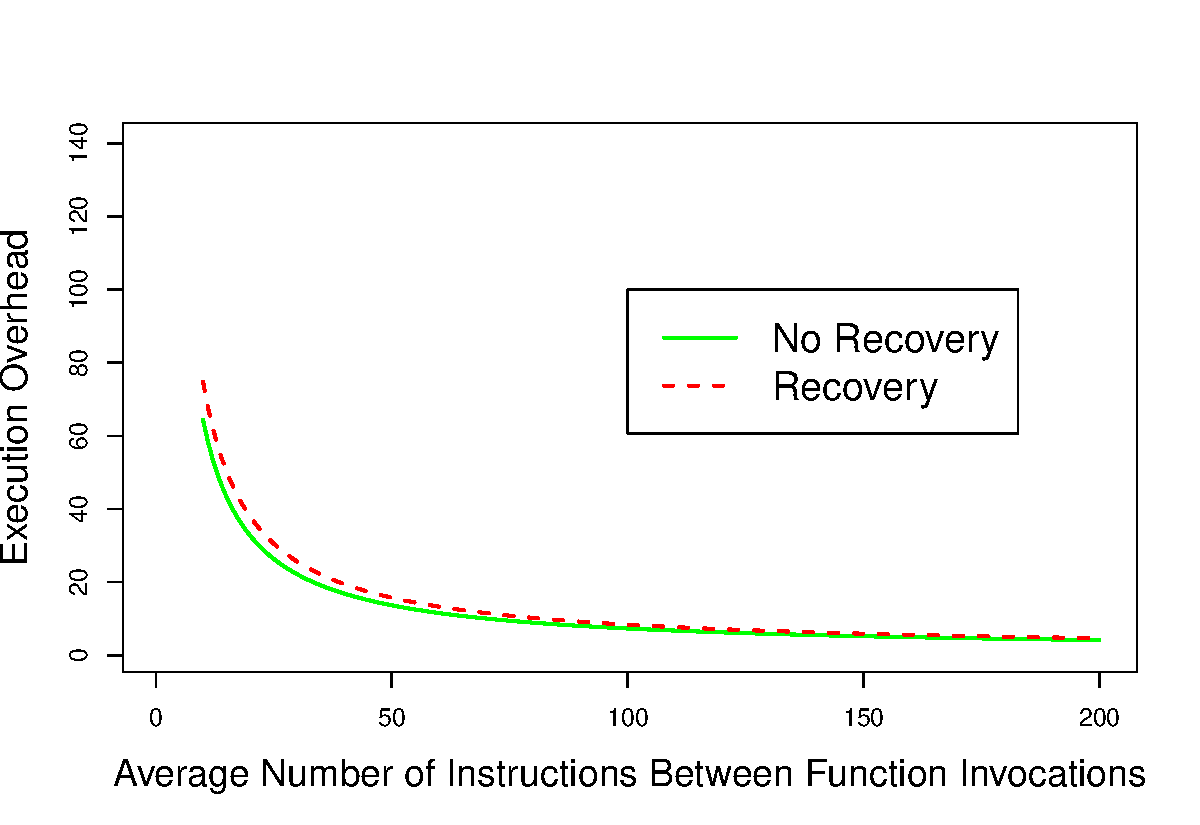
\includegraphics[width=0.47\textwidth]{figures/speed_overhead_line_chart_v1.pdf}
\vspace{5pt}
\caption{Execution Overhead}
\label{fig:speed_overhead}
\end{figure}

\subsection{Physical Hardware}
To validate our approach on physical hardware, we emulate the occurrence of SEUs by flipping random bits in the target SRAM area. To perform auditable test runs, we developed an AVR application which continuously generates an increasing integer sequence, which is then sent to the UART interface at a controllable speed. A Python program running on a desktop is used to receive the sequence and observe the impact of flipped bits by monitoring the continuity of the sequence. A timer interrupt is used to trigger the occurrence of SEUs. The interrupt service routine generates a random address within the range of the top of the stack and the end of RAM space, excluding the stack frame of the current interrupt, and then flips the bit at this location. The bit flip frequencies are set to 39062Hz, 4878Hz, 609Hz, 153Hz, and 38Hz\footnote{These frequencies are derived from the built-in timer prescaler of the Atmega644 at values of 1, 8, 64, 256, and 1024, respectively}. An Atmega644 microprocessor is used in our experiments.

We declare (observable) failure when one of the following two situations occurs: (i) The AVR application stops generating integers; or (ii) the integer sequence received by the Python program becomes discontinuous. We monitor the integer sequence and record the maximum count before failure. The experimental results are summarized in Figure \ref{fig:exp1_result}. The x-axis represents SEU injection frequency, and the y-axis represents the maximum count received by the Python program. The figure shows that as SEU injection frequency increases, running time to failure decreases. This is explained as follows: As SEU injection frequency increases, the probability that an SEU occurs in a critical area increases. When the frequency is extremely high (e.g. approximate 10 MHz), the program can hardly send any values. However, the observed SEU occurrence rate in outer space is approximately $10^{-6}SEU/bit$-$Day$~\cite{underwood1992observations}. Given that the total RAM size of an Atmega644 is 4K Bytes, the expected SEU occurrence rate for an Atmega644 is 0.0032 SEU/day, which is significantly lower than the lowest frequency (9765.625 SEU/second) that we used. This situation would be extremely rare in real scenarios.

%We declare (observable) failure when one of the following two situations occurs: (i) The AVR application stops generating the integers; or (ii) the integer sequence received by the Python program becomes noncontinuous. We monitor the integer sequence and record the maximum count before failure. In the experiment, the Atmega644 microprocessor runs at $10^7$Hz. The error insertion frequencies are set to $10^7$Hz, $1.25*10^6$Hz, $1.5625*10^5$Hz, $39062.5$Hz, $9765.625$Hz.\footnote{derived from the built-in timer prescaler of Atmega644, at 1, 8, 64, 256, 1024, respectively} The \textit{delay} function is used to control integer sequence generation frequency, which is set to 1Hz, 10Hz, 100Hz, and 1000Hz. The experimental results are summarized in Figure \ref{fig:exp1_result}. The x-axis represents the error insertion frequency, and the y-axis represents the maximum count received by the Python program. The figure shows that given the same error insertion frequency, as the program running speed increases, the maximum integer received by the Python program increases. This is because that since the probability of SEUs occur on critical area is fixed, faster program running speed will generate more numbers. Given the same integer generation frequency, as the error insertion frequency increases, the maximum correct number received by the Python program decreases. This is explained as follows: as the error insertion frequency increases, the probability that SEUs occur on critical area increases. When the error insertion frequency is extremely high, the program can hardly send anything. However, the observed SEU occurrence rate is approximate $10^{-6}SEU/bit$-$Day$ in the outer space~\cite{underwood1992observations}, which is significantly lower than our test frequencies.

\begin{figure}
\centering
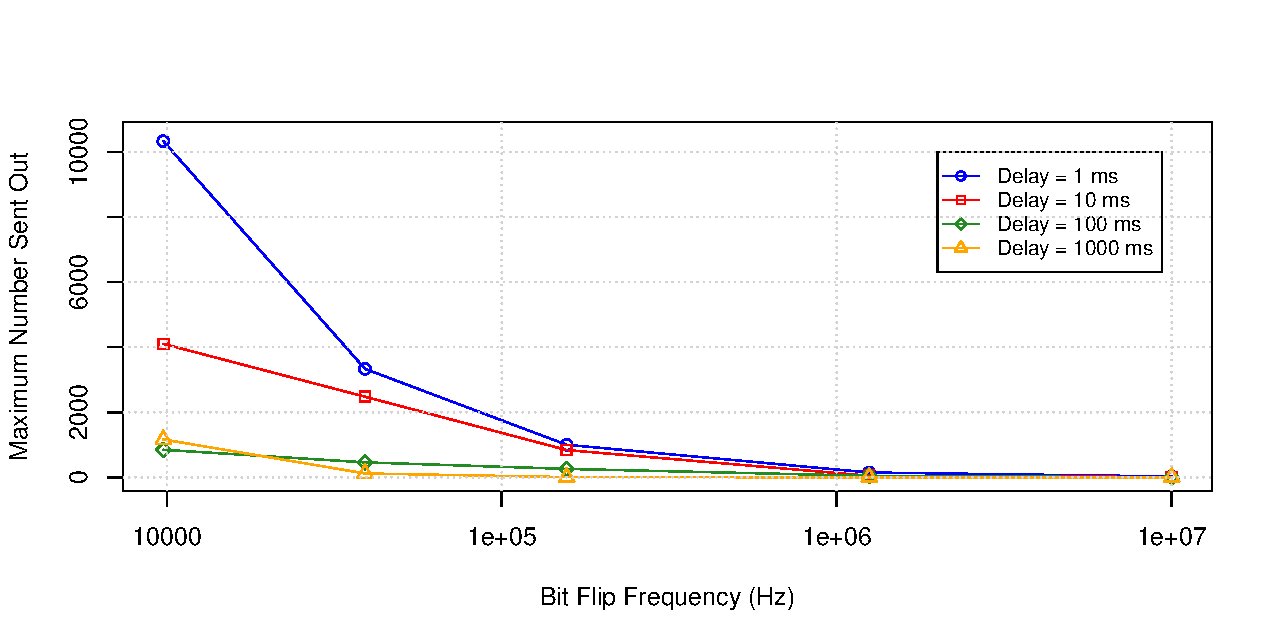
\includegraphics[scale=0.4]{figures/experiment1.pdf}
\caption{SEU Experiment Results}
\vspace{5pt}
\label{fig:exp1_result}
\end{figure}




\section{Conclusion}\label{sec:conclusion}

The single event upset is among the most common types of system faults introduced by radiation, posing significant risk to spacecraft embedded systems. Modern approaches to guarding against such faults often introduce additional hardware to detect and correct SEU errors in target systems. In this paper, we present a software-only approach to protecting embedded system memory from SEUs. 

Our approach focuses on the system stack, which is the most important and dynamic region in memory. The stack is protected by injecting auxiliary assembly code within the target program. The prototype implementation is based on the AVR architecture, but is easily adapted to other architectures. Analytical and experimental results show that our approach detects and corrects SEU errors as expected. 

A study on protection efficacy has been provided, analyzing the probability of successful SEU protection as SEU frequency is increased. Experimental results for both ROM and execution (speed) overhead have been provided, using three applications with different degrees of stack dynamism. Since the size of the injected code is fixed, space overhead depends only on the number of functions in the target program and the size of each function. Speed overhead depends largely on function frame size and stack dynamism, as well as the occurrence rate of SEUs. Results show that for typical programs, our approach achieves a stack protection success rate of over 99\%.

{\bf Future Work}. Our future work follows four tracks. The first is focused on protecting global portions of RAM. In our current design, we ignore the .data and .bss sections used to store global and static variables. Since global and static variables are commonly used in embedded applications, introducing protection to these sections will improve the utility of our approach. The second involves introducing compression to the stack frame copy process. In our current design, stack frames are directly copied. Although compression will increase ROM and execution (speed) overhead, RAM usage and the probability that the stack frame copies are affected by SEUs can be reduced. Third, we plan to extend our approach to other GCC optimization levels. In the current design, optimization level option -O0 is used. However, other options, such as -O2 or -Os, are frequently used by developers. Applying our design to other levels involves studies on assembly code generated with other optimization levels and will further improve the utility of our approach. Finally, we plan to add support for external RAM. Internal RAM is a valuable resource in embedded systems. Our approach uses the internal RAM to store the stack frame copies, reducing the RAM space available for the target program. Adding external RAM can provide more space to store stack frame copies and offers more flexibility in future designs.

%Third, we plan to study scenarios where SEU occurrence is not uniformly distributed. In this paper, a uniform distribution is assumed. However, in real systems, the distribution depends on the altitude and angle of the device towards the sun.
\vspace{-15pt}
\section{Acknowledgments}\label{sec:acknowlegments}
\vspace{-10pt}
This work is supported by the National Science Foundation through awards CNS-0745846 and CNS-1126344, and the City of Aiken, SC.

%
% The following two commands are all you need in the
% initial runs of your .tex file to
% produce the bibliography for the citations in your paper.

{\footnotesize \bibliographystyle{acm}
\bibliography{./sigproc}}

% sigproc.bib is the name of the Bibliography in this case
% You must have a proper ".bib" file
%  and remember to run:
% latex bibtex latex latex
% to resolve all references
%
% ACM needs 'a single self-contained file'!
%

\end{document}
